\documentclass[11pt]{article}
\usepackage[a4paper,margin=21mm]{geometry}
\usepackage{fontspec}
\setmainfont{Latin Modern Roman}
\newfontfamily\CJKfont{Noto Serif CJK SC}
\XeTeXlinebreaklocale "zh"
\XeTeXlinebreakskip=0pt plus 1pt
\usepackage{amsmath,amssymb,amsthm,amscd,graphicx,color}
\usepackage{xurl}
\usepackage[unicode,hidelinks]{hyperref}
\allowdisplaybreaks
\setlength\emergencystretch{3em}
\numberwithin{equation}{section}

\numberwithin{equation}{section}

\newtheorem{Theorem}{Theorem}[section]
\newtheorem{Corollary}[Theorem]{Corollary}
\newtheorem{Lemma}[Theorem]{Lemma}
\newtheorem{Proposition}[Theorem]{Proposition}
 { \theoremstyle{definition}
\newtheorem{Definition}[Theorem]{Definition}
\newtheorem{Note}[Theorem]{Note}
\newtheorem{Example}[Theorem]{Example}
\newtheorem{Remark}[Theorem]{Remark} }

\newcommand{\norme}[1]{\left\Vert #1\right\Vert}
\newcommand{\abss}[1]{\left\vert #1 \right\vert}
\newcommand{\rcap}{\tikz[scale = 0.3] \draw[->] (0,0) arc(180:0:1);}
\newcommand{\rcup}{\tikz[scale = 0.3] \draw[->] (0,0) arc(-180:0:1);}
\newcommand{\lcap}{\tikz[scale = 0.3] \draw[<-] (0,0) arc(180:0:1);}
\newcommand{\lcup}{\tikz[scale = 0.3] \draw[<-] (0,0) arc(-180:0:1);}
\newcommand{\undC}{\underline{\mathcal{C}}}
\newcommand{\undD}{\underline{\mathcal{D}}}
\newcommand{\undM}{\underline{\mathcal{M}}}
\newcommand{\undO}{\underline{\mathcal{O}}}

\usepackage{tikz}
\usetikzlibrary{arrows,decorations.pathmorphing,positioning}
\usepackage{mathrsfs}
\usepackage{bm}

\newcommand{\pullback}[5]{\begin{tikzpicture}[scale = #5, baseline]
\node (P) at (0,1) {#1}; \node (X) at (0,0) {#3}; \node (Y) at (1,1) {#2}; \node (S) at (1,0) {#4};
\draw [->] (P) -- (X); \draw [->] (P) -- (Y); \draw [->] (X) -- (S); \draw [->] (Y) -- (S);
\node [below right = -10pt of P] {$\lrcorner$};
\end{tikzpicture}}
\newcommand{\pushout}[6]{\begin{tikzpicture}[xscale = #5, yscale = #6, baseline]
\node (P) at (0,1) {#1}; \node (X) at (0,0) {#3}; \node (Y) at (1,1) {#2}; \node (S) at (1,0) {#4};
\draw [->] (P) -- (X); \draw [->] (P) -- (Y); \draw [->] (X) -- (S); \draw [->] (Y) -- (S);
\node [above left = -10pt of S] {$\ulcorner$};
\end{tikzpicture}}
\newcommand{\Kaufhoriz}{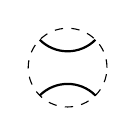
\begin{tikzpicture}[scale = 0.5, baseline = -3pt]
\draw[dashed] (0,0) circle(1);
\draw[thick] (45:1) arc (-45:-135:1);
\draw[thick] (-45:1) arc (45:135:1);
\end{tikzpicture}}
\newcommand{\Kaufvert}{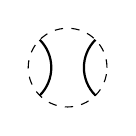
\begin{tikzpicture}[scale = 0.5, baseline = -3pt]
\draw[dashed] (0,0) circle(1);
\draw[thick] (45:1) arc (135:225:1);
\draw[thick] (135:1) arc (45:-45:1);
\end{tikzpicture}}
\newcommand{\Kauftresse}{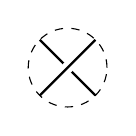
\begin{tikzpicture}[scale = 0.5, baseline = -3pt]
\draw[dashed] (0,0) circle(1);
\draw[thick] (-45:1) -- (135:1) node[fill, color= white, pos = 0.5, circle, scale = 0.45]{};
\draw[thick] (45:1) -- (-135:1);
\end{tikzpicture}}
\newcommand{\Kaufcirc}{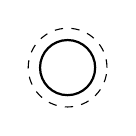
\begin{tikzpicture}[scale = 0.5, baseline = -3pt]
\draw[dashed] (0,0) circle(1);
\draw[thick] (0,0) circle(0.7);
\end{tikzpicture}}
\newcommand{\Kaufvide}{\begin{tikzpicture}[scale = 0.5, baseline = -3pt]
\draw[dashed] (0,0) circle(1);
\end{tikzpicture}}
%\newcommand{\Kaufrel}{\[ \Kauftresse \ = q \Kaufvert\ +q^{-1} \Kaufhoriz \qquad \text{and} \qquad \Kaufcirc \ = \big({-}q^2-q^{-2}\big) \Kaufvide\ . \]}
\newcommand{\braiding}{
\begin{tikzpicture}[scale = 0.3, baseline]
\draw [thick] (1,0) -- (0,1);
\draw[line width = 4pt, color = white] (0,0) -- (1,1);
\draw [thick] (0,0) -- (1,1);
\end{tikzpicture}}
\newcommand{\twist}{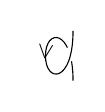
\begin{tikzpicture}[scale = 0.35, baseline = 5pt]
\draw (1,0.1) .. controls (1,2) and (0,2) .. (0,1) node[fill, color= white, pos = 0.21, circle, scale = 0.55]{} node[pos = 0.95, sloped]{\footnotesize $<$};
\draw (1,1.9) .. controls (1,0) and (0,0) .. (0,1);
\end{tikzpicture}\ }
\newcommand{\unortwist}{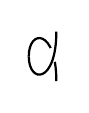
\begin{tikzpicture}[scale = 0.35, baseline = 5pt]
\draw[thick] (1,0.1) .. controls (1,2) and (0,2) .. (0,1) node[fill, color= white, pos = 0.21, circle, scale = 0.55]{};
\draw[thick] (1,1.9) .. controls (1,0) and (0,0) .. (0,1);
\end{tikzpicture}}
\newcommand{\ribtwist}{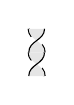
\begin{tikzpicture}[yscale = 0.15, xscale = 0.2, baseline = 5pt]
\draw[thick] (1,0) .. controls (1,1) and (0,1) .. (0,2) node[fill, color= white, pos = 0.5, circle, scale = 0.5]{};
\fill[gray!20] (0,0) .. controls (0,1) and (1,1) ..(1,2)-- (0,2) .. controls (0,1) and (1,1) .. (1,0) -- (0,0);
\draw (0,0) .. controls (0,1) and (1,1) .. (1,2);
\begin{scope}[yshift = 2cm]
\draw[thick] (1,0) .. controls (1,1) and (0,1) .. (0,2) node[fill, color= white, pos = 0.5, circle, scale = 0.5]{};
\fill[gray!20] (0,0) .. controls (0,1) and (1,1) ..(1,2)-- (0,2) .. controls (0,1) and (1,1) .. (1,0) -- (0,0);
\draw (0,0) .. controls (0,1) and (1,1) .. (1,2);
\end{scope}
\end{tikzpicture}\ }
\newcommand{\halftwist}{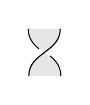
\begin{tikzpicture}[yscale = 0.3, xscale = 0.4, baseline = 2pt]
\draw[thick] (1,0) .. controls (1,1) and (0,1) .. (0,2) node[fill, color= white, pos = 0.5, circle, scale = 0.5]{};
\fill[gray!20] (0,0) .. controls (0,1) and (1,1) ..(1,2)-- (0,2) .. controls (0,1) and (1,1) .. (1,0) -- (0,0);
\draw (0,0) .. controls (0,1) and (1,1) .. (1,2);
\end{tikzpicture}\ }
\newcommand{\doubleloop}{
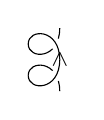
\begin{tikzpicture}[xscale = 0.4, yscale = 0.2, baseline = 5pt]
\draw (1,0) .. controls (1,2) and (0,2) .. (0,1) node[fill, color= white, pos = 0.21, circle, scale = 0.45]{};
\draw (1,2) .. controls (1,0) and (0,0) .. (0,1);
\begin{scope}[yshift = 2cm]
\draw (1,2) .. controls (1,0) and (0,0) .. (0,1) node[fill, color= white, pos = 0.21, circle, scale = 0.45]{};
\draw (1,0) .. controls (1,2) and (0,2) .. (0,1) node[pos = 0, sloped]{\footnotesize $>$};
\end{scope}
\end{tikzpicture}\ }
\newcommand{\St}{\operatorname{St}}
\newcommand{\halft}{{\operatorname{ht}}}
\newcommand{\Ind}{\operatorname{Ind}}
\newcommand{\Free}{\operatorname{Free}}
\newcommand{\colim}{\operatorname{colim}}
\newcommand{\Hom}{\operatorname{Hom}}
\newcommand{\Fun}{\operatorname{Fun}}
\newcommand{\End}{\operatorname{End}}
\newcommand{\undHom}{\underline{\operatorname{Hom}}}
\newcommand{\undEnd}{\underline{\operatorname{End}}}
\newcommand{\im}{\operatorname{im}}
\newcommand{\coker}{\operatorname{coker}}
\newcommand{\bmrhd}{\bm{\triangleright}}
\newcommand{\bmotimes}{\bm{\otimes}}
\newcommand{\Oqcomfin}{\Oq\text{-}{\rm comod}^{\rm fin}}
\newcommand{\Oqcom}{\Oq\text{-}{\rm comod}}
\newcommand{\Oq}{\mathcal{O}_{q^2}({\rm SL}_2)}
\newcommand{\Uq}{\mathcal{U}_{q^2}(\mathfrak{sl}_2)}
\newcommand{\Uqmodfin}{\Uq\text{-}{\rm mod}^{\rm fin}}
\newcommand{\Uqmod}{\Uq\text{-}{\rm mod}}

\tikzset{leftymissy/.style={path picture={\draw[black](path picture bounding box.north west) -- (path picture bounding box.north east) -- (path picture bounding box.south east) -- (path picture bounding box.south west);}}}
\tikzset{rightymissy/.style={path picture={\draw[black](path picture bounding box.south east) -- (path picture bounding box.south west) -- (path picture bounding box.north west) -- (path picture bounding box.north east);}}}
\tikzset{topydowny/.style={path picture={\draw[black](path picture bounding box.north west) -- (path picture bounding box.north east)
(path picture bounding box.south east) -- (path picture bounding box.south west);}}}


\makeatletter\newlabel{SectMultiEdges}{{4}{}{Original source locator}{}{}}\makeatother
\makeatletter\newlabel{rmkChoiceCutting}{{4.34}{}{Original source locator}{}{}}\makeatother
\begin{document}
\begin{center}\Large Generic-parameter stated skein algebras represent internal empty-object endomorphism comodule algebras for compact oriented surfaces with a distinguished boundary edge\end{center}
\noindent\textbf{Stable ID:} 1246\quad\textbf{Author:} Benjamin Haïoun\par
\noindent\textbf{Work:} Relating Stated Skein Algebras and Internal Skein Algebras\par
\noindent\textbf{Source:} \url{https://sigma-journal.com/2022/042/}\par
\noindent\textbf{Version:} Official SIGMA 18 (2022) article 042, DOI 10.3842/SIGMA.2022.042; journal PDF and native TeX acquired 2026-09-30, exact bytes pinned by SHA256\par
\noindent\textbf{Rights:} CC BY 4.0. Authors retain copyright. \url{https://creativecommons.org/licenses/by/4.0/}. Reuse and typesetting adaptation; original language and mathematical content preserved.\par
\noindent\textbf{Difficulty (prior selection preserved):} {\CJKfont H2: The proof identifies stated boundary relations with naturality for quantum-group caps and cups, then constructs an explicit inverse on simple comodules and checks independence of the chosen tangle representative. It extends the resulting representing transformation through free cocompletion and derives the multiplication from internal evaluation and composition. The boundary orientation conventions are essential to obtaining the usual stacking product rather than its braided opposite.}\par
\medskip\noindent\textbf{Editorial boundary note (not author text):} Selected generic-parameter first-edge Theorem1.1/Theorem3.4 together with full multiplication Proposition3.5: compact oriented surface and specified boundary edge, seen at the right for stated tangles and left for the internal action; ground Q(q\textasciicircum{}(1/2)) or C with nonzero non-root-of-unity parameter. Full unusual coribbon convention, quantum-group/coaction/Temperley–Lieb/stated relations, free cocompletion and evaluation/composition definitions are retained. Complete current St map, all cap/cup coefficients and diagrams, naturality, explicit inverse/representative checks and full multiplication/extension proof are unchanged. Established quantum-group semisimplicity, tangle generation, stated relations/bigon and cocompletion results stay precisely cited prerequisites. Multiple-edge/right-action/excision variants and auxiliary components receive no extra counts. All retained author diagrams are native editable TikZ; no private style or formula transformation.\par
\noindent\textbf{External original reference SectMultiEdges:} Original unselected multi-edge/right-action commentary section4, native1555–2384; not a required new first-edge proof\par
\noindent\textbf{External original reference rmkChoiceCutting:} Original future alternative state-matching commentary, native2374–2382, not a selected first-edge core premise\par
\medskip\hrule\medskip\noindent\textbf{Author text begins below.}\par
\setcounter{section}{1}\setcounter{Theorem}{0}
% Original source lines 206--210
\subsection*{Relating stated skein algebras and internal skein algebras} When $\mathcal{V} = \Oqcomfin$, we show that these two algebras are isomorphic as $\Oq$-comodule-algebras. This result was already known as folklore and stated in a slightly weaker form (only as algebras in $\rm Vect$) in \cite[Theorem~4.4]{LeYu}, \cite[Theorem~9.1]{LeSikora} and \cite[Remark 2.21]{Gunningham}. Note that in their context the isomorphism a priori cannot be improved to an $\Oq$-comodule-algebra isomorphism because of the product inversion coming from seeing the boundary edge at the right. On the other hand, both algebras are known to be isomorphic to the Alekseev--Grosse--Schomerus moduli algebras, which are deformation quantizations of the representation variety of a punctured surface in the direction of the Fock--Rosly Poisson structure. In \cite[Theorem~5.3]{Faitg} and \cite{Korinman} the authors provide an $\Oq$-comodule algebra isomorphism between these AGS algebras and stated skein algebras. In \cite[Section~7]{BBJ} the authors provide an isomorphism between AGS algebras and internal skein algebras. Note though that one does not see the braided opposite algebra structure through these isomorphisms, and it might be that one deforms the representation variety in the direction of the opposite Poisson structure. Section~\ref{SectRelation} gives a more direct proof of the isomorphism using only skein theory.
\begin{Theorem}[Theorem~\ref{thmRelation}]
For $\mathcal{V} = \Oqcomfin$ and $\Sigma$ a compact oriented surface with a~boundary edge $e$ seen at the right for stated skein algebras, and at the left for internal skein algebras, one has an isomorphism of $\Oq$-comodule-algebras $A_\Sigma \simeq \mathscr{S}(\Sigma)$.
\end{Theorem}
We explicitly give the natural isomorphisms $\St_W\colon\Hom_{{\rm Sk}_\mathcal{V}(\Sigma)}(W\rhd\varnothing,\varnothing) \tilde{\to} \Hom_{\mathcal{V}}(W,\mathscr{S}(\Sigma))$ exhi\-bi\-ting $\mathscr{S}(\Sigma)$ as the internal endomorphism algebra of the empty set in ${\rm Sk}_\mathcal{V}(\Sigma)$, without relying on excision properties. We only give $\St_W$ for $W\in {\rm Sk}_\mathcal{V}(\mathbb{R}^2)$ a well-ordered set of points coloured by the standard corepresentation $V$ of basis $v_+$,~$v_-$~-- equivalently, an object of the Temperley--Lieb full subcategory ${\rm TL}$~-- which is sufficient as these objects generate the whole category under colimits. This natural isomorphism is the expected one. Any morphism in the left hand side can be described by a~(linear combination of) tangle $\alpha$ with $n$ boundary points coloured by $V$. Then $\St_{V^{\otimes n}}(\alpha)\colon V^{\otimes n} \to \mathscr{S}(\Sigma)$ maps a simple tensor $v_{\varepsilon_1}\otimes\cdots \otimes v_{\varepsilon_n}$ to the tangle~$\alpha$ with states $\varepsilon_1,\dots,\varepsilon_n$ from top to bottom.

\setcounter{section}{1}
% Original source lines 238--425
\section{Preliminaries}\label{SectPreliminaries}
We recall basic facts about the quantum groups $\Oq$ and $\Uq$, and the needed constructions and properties of skein categories in~\cite{Cooke} and of stated skein algebras in \cite{Cos}. We finish with a slight modification of the construction of internal skein algebras of \cite{Gunningham}. Let $k$ be either $\mathbb{Q}\big(q^{\frac{1}{2}}\big)$ or $\mathbb{C}$ with $q^{\frac{1}{2}} \in \mathbb{C}^\times$ generic, i.e., not a root of unity. We work in the symmetric monoidal (2,1)-category ${\rm Cat}_k$ of small $k$-linear categories, $k$-linear functors and natural isomorphisms, where the tensor product $\mathcal{C} \otimes \mathcal{D}$ has objects $\operatorname{Ob}(\mathcal{C}) \times \operatorname{Ob}(\mathcal{D})$ and morphisms $\Hom_{\mathcal{C} \otimes \mathcal{D}}((c,d),(c',d')) := \Hom_\mathcal{C}(c,c') \otimes_k \Hom_\mathcal{D}(d,d')$.

\subsection[The coribbon Hopf algebra O\_\{q\textasciicircum{}2\}(SL\_2)]
{The coribbon Hopf algebra $\boldsymbol{\Oq}$}\label{SectRibCat}

We recall the definition of the coribbon Hopf algebra $\Oq$, its categories of right comodules and their links with left $\Uq$-modules.
\begin{Definition}
The coribbon Hopf algebra $\Oq$ is the free $k$-algebra with
(one should read the matrix equations component-wise, and the tensor product of matrices should be computed as a usual matrix product with tensor products of coefficients instead of products)
\begin{alignat*}{3}
& \text{generators}\colon&& a,\ b,\ c,\ d,&
\\
& \text{relations}\colon&& ca = q^2ac,\quad db = q^2bd,\quad ba = q^2ab,\quad dc = q^2cd,&
\\
&&& bc = cb,\quad ad - q^{-2}bc = 1\quad \text{and}\quad da - q^2cb = 1,&
\\
&\text{coproduct}\colon&&\Delta\begin{pmatrix} a & b \\[-.5ex] c & d \end{pmatrix}
= \begin{pmatrix} a & b \\[-.5ex] c & d \end{pmatrix} \otimes \begin{pmatrix} a & b \\[-.5ex] c & d \end{pmatrix}\!,&
\\
& \text{counit}\colon&& \varepsilon \begin{pmatrix} a & b \\[-.5ex] c & d \end{pmatrix}
= \begin{pmatrix} 1& 0 \\[-.5ex] 0 & 1\end{pmatrix}\!,&
\\
& \text{antipode}\colon&& S \begin{pmatrix} a & b \\[-.5ex] c & d \end{pmatrix}
= \begin{pmatrix} d & -q^2b \\[-.5ex] -q^{-2}c & a \end{pmatrix}\!,&
\\
&\text{co-}R\text{-matrix}\colon&& R \begin{pmatrix}
a \otimes a & a \otimes b & b \otimes a & b \otimes b
\\
a \otimes c & a \otimes d & b \otimes c & b\otimes d\\ c\otimes a & c\otimes b & d \otimes a & d\otimes b\\ c\otimes c & b\otimes d & d\otimes c & d\otimes d \end{pmatrix}
=\begin{pmatrix} q& 0 & 0 & 0\\ 0 & q^{-1} & q-q^{-3} & 0\\ 0 & 0 & q^{-1}&0\\ 0 & 0 & 0 & q \end{pmatrix}\!,&
\\
& \text{coribbon functional}\colon \quad && \theta \begin{pmatrix} a & b \\[-.5ex] c & d \end{pmatrix}
= \begin{pmatrix} -q^3 & 0 \\[-.5ex] 0 & -q^3 \end{pmatrix}\!.&
\end{alignat*}
\end{Definition}

\begin{Remark}
We took the coribbon functional so that the twist on a comodule $V$ is given by $\theta_V\colon V \overset{\Delta_V}{\to} V \otimes H \overset{{\rm Id}_V \otimes \theta}{\to} V$. In the literature (see \cite{Wakui} for the coribbon case, or \cite{Kassel} for the ribbon case), the coribbon functional is defined to be $\theta^{-1}$ in our definition.
Moreover, we use here an unusual coribbon functional, which arises naturally on the stated skein algebra of the bigon in Section~\ref{SectStatedSkein}. It is studied in \cite{Tingley} where the author proves that it gives precisely the Kauffman-bracket relation under the Reshetikhin--Turaev functor, whereas the usual coribbon functional gives relations which differ by a sign, and give the Jones polynomial after writhe renormalisation.\looseness=-1
\end{Remark}

\begin{Definition}\label{defOqcomods}
The quantum plane $\mathbb{A}_{q^2}^2$ is the free $k$-algebra generated by $x$ and $y$ modulo the relation $yx = q^2xy$. It is a right $\Oq$-comodule algebra with $\Delta \left(\begin{smallmatrix} x&y \end{smallmatrix}\right) = \left(\begin{smallmatrix} x&y \end{smallmatrix}\right) \otimes \left( \begin{smallmatrix} a & b \\ c & d \end{smallmatrix}\right)$ on generators.

Its subspace of homogeneous polynomials of degree $n$ forms a sub-comodule which we denote by~$V_n$.
In particular the generators span the comodule $V_1$ which we abbreviate $V$ and call the standard co-representation of $\Oq$. It is more conventional to call its basis $v_+ = x$ and $v_- = y$. This comodule is self dual. The left dual $V^*$ of $V$ has basis $v_+^*$ and $v_-^*$, and one has an isomorphism of $\Oq\text{-comodules}$
\begin{gather*}
\varphi \colon \
\begin{cases}
V \to V^*,
\\
v_+ \mapsto -q^{\frac{5}{2}} v_-^*,
\\[.5ex]
v_- \mapsto q^{\frac{1}{2}}v_+^*.
\end{cases}
\end{gather*}
\end{Definition}

{\sloppy\begin{Proposition}[{\cite[Section~4.2.1]{Klimyk}}]\label{propOqSemiSimple}
The $\Oq$-comodules $V_n,\ n \in \mathbb{N}$, are all the simple $\Oq$-comodules. Moreover, the categories $\Oq\text{-}{\rm comod}$ and $\Oq\text{-}{\rm comod}^{\rm fin}$ are semi-simple.
\end{Proposition}}

\begin{Definition}
The Hopf algebra $\Uq$ is the free $k$-algebra with:
\begin{alignat*}{3}
& \text{generators}\colon\quad  &&E,\,F,\,K,&
\\
&\text{relations}\colon && KE=q^4EK, \quad KF=q^{-4}FK,\quad  EF-FE = \frac{K-K^{-1}}{q^2-q^{-2}},&
\\
&\text{coproduct}\colon &&\Delta (K) = K \otimes K,\quad \Delta (E) = 1\otimes E+E\otimes K,\quad \Delta (F) = K^{-1}\otimes F + F\otimes 1,&
\\
& \text{counit}\colon && \varepsilon(K)=1,\quad\varepsilon(E)=\varepsilon(F)=0,&
\\
& \text{antipode}\colon && S(K) = K^{-1},\quad S(E) = -EK^{-1},\quad S(F) =-KF.&
\end{alignat*}
\end{Definition}

\begin{Definition}
The left $\Uq$-module $V_{\pm,n}$ is the vector space of dimension $n+1$ with action:
\begin{gather*}
 K=\pm \setlength{\arraycolsep}{1.5pt}\begin{pmatrix}
 q^{2n} & 0& \cdots & 0 \\ 0& q^{2(n-2)} &\ddots &\vdots \\ \vdots &\ddots &\ddots&0 \\ 0 &\cdots&0& q^{-2n}\end{pmatrix}\!,\qquad
 E=\setlength{\arraycolsep}{2.5pt}\begin{pmatrix}
 0 & [n]_{q^2}& & 0 \\ & \ddots &\ddots & \\ \vdots & &\ddots&[1]_{q^2} \\ 0 & \cdots & & 0\end{pmatrix}\!,\\
 F=\setlength{\arraycolsep}{2.5pt}\pm \begin{pmatrix}
 0 & & \cdots & 0 \\ {[1]_{q^2}} & \ddots & & \vdots\\ & \ddots&\ddots& \\ 0 & & [n]_{q^2}& 0\end{pmatrix}\!,
 \end{gather*}
 where $ [n]_{q^2} = \frac{q^{2n}-q^{-2n}}{q^2-q^{-2}}$.

The modules of the form $V_{+,n}$ are called of type 1, and the others are discarded here. The mo\-du\-le~$V_{+,1}$ is denoted by $V$ and called the standard representation of $\Uq$.
A module $W$ is called locally finite (of type 1) if $\forall w \in W$, $\Uq \cdot w$ is finite-dimensional (and isomorphic to some $V_{+,n}$).
\end{Definition}

\begin{Proposition}[{\cite[Theorem~VII.2.2]{Kassel}}]
The $\Uq$-modules $V_{\pm,n},\ n \in \mathbb{N}$ are all the locally finite simple $\Uq$-modules. Moreover, the categories $\Uq\text{-}{\rm mod}^{\rm lf}$ and $\Uq\text{-}{\rm mod}^{\rm fin}$, of respectively locally finite and finite-dimensional $\Uq$-modules of type $1$, are semi-simple.
\end{Proposition}

\begin{Definition}
We can define a dual pairing, namely a non-degenerate bilinear form
\[
\langle \cdot,\cdot\rangle \colon \  \Uq \otimes \Oq \to k
\] satisfying $\langle x, y.y'\rangle = \langle x_{(1)},y\rangle \langle x_{(2)},y'\rangle$, $\langle x.x', y\rangle = \langle x,y_{(1)}\rangle \langle x',y_{(2)}\rangle$, $\langle x,1\rangle = \varepsilon(x)$, $\langle 1,y\rangle = \varepsilon(y)$ and $\langle S(x),y\rangle = \langle x,S(y)\rangle$. It is given on generators by
\begin{gather*}
 \left\langle K,\begin{pmatrix}a&b\\c&d \end{pmatrix} \right\rangle =
 \begin{pmatrix}q^2&0\\0&q^{-2} \end{pmatrix}\!, \qquad \!
 \left\langle E,
 \begin{pmatrix}a&b\\c&d \end{pmatrix} \right\rangle =
 \begin{pmatrix}0&1\\0&0 \end{pmatrix}\!,\qquad \!
 \left\langle F,\begin{pmatrix} a&b\\c&d \end{pmatrix}\right\rangle =
 \begin{pmatrix}0&0\\1&0 \end{pmatrix}\!.
 \end{gather*}
 A right $\Oq$-comodule structure on some vector space $W$ induces a left $\Uq$-module structure by $x\cdot w = w_{(1)}. \langle x,w_{(2)} \rangle$, $x \in \Uq$, $w\in W$.
\end{Definition}

\begin{Proposition}[{\cite[equation~(3.3), p.~126]{Abe}, \cite[Theorem~7.9]{Takeuchi}}]\label{propOqcomodUqmod}
This correspondence induces equivalences of categories $\Oq\text{-}{\rm comod}^{\rm fin}\simeq \Uq\text{-}{\rm mod}^{\rm fin}$ and $\Oq\text{-}{\rm comod} \simeq \Uq\text{-}{\rm mod}^{\rm lf}$.

The simple comodules $V_n$ are mapped on the simple modules $V_{+,n}$.
\end{Proposition}

Note that this correspondence also preserves the monoidal (and actually ribbon, though using an unusual twist on $\Uqmod$) structure. In the following, we will mostly adopt the point of view of comodules over $\Oq$, because there are fewer conditions to ask, the braided and ribbon structure of $\Oq$ is algebraic and not ``topological'', and it has a geometric description using stated skein algebras.


\subsection{Skein categories}\label{SectSkCat}
Tangle invariants obtained from a $k$-linear ribbon category $\mathcal{V}$ are defined in \cite[Section~I.2]{Turaev}. They can be extended to give tangle invariants on any oriented surface $\Sigma$ by local relations, and produce the skein category of the surface ${\rm Sk}_\mathcal{V}(\Sigma)$, see \cite{Walker}. We will use and recall their boundary structure and excision properties, see \cite{Cooke}.

\begin{Definition}
Let $[n]$ denote the set of $n$ points $\{1,\ldots,n\} \times \{0\}$ in $\mathbb{R}^2$, equipped with blackboard framing (coming out of the page when we draw ribbon graphs as below) and ${\rm Ribbon}_\mathcal{V}$ the category whose objects are framed oriented $\mathcal{V}$-coloured points of $\mathbb{R}^2$ of the form $[n]$, and morphisms ribbon graphs (i.e., $\mathcal{V}$-coloured oriented framed tangles with coupons coloured by morphisms) between them in $\mathbb{R}^2\times[0,1]$.
\end{Definition}
$$
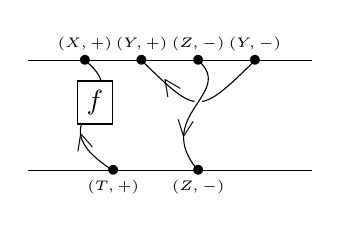
\begin{tikzpicture}[baseline = 15pt, yscale = 0.7, xscale = 1.2]
\draw (0,2) -- (3,2) node[pos = 0.2]{\small $\bullet$} node[pos = 0.2, above]{\tiny $(X,+)$} node[pos = 0.4]{\small $\bullet$} node[pos = 0.4, above]{\tiny $(Y,+)$} node[pos = 0.6]{\small $\bullet$} node[pos = 0.6, above]{\tiny $(Z,-)$} node[pos = 0.8]{\small $\bullet$} node[pos = 0.8, above]{\tiny $(Y,-)$};
\draw (0,0) -- (3,0) node[pos = 0.3]{\small $\bullet$} node[pos = 0.3, below]{\tiny $(T,+)$} node[pos = 0.6]{\small $\bullet$} node[pos = 0.6, below]{\tiny $(Z,-)$};
\draw (0.9,0) .. controls (0,1) and (1.2,1.2) .. (0.6,2) node[pos=0.2, sloped]{$<$} node [pos = 0.6, rectangle, draw, fill=white]{$f$};
\draw (1.2,2) .. controls (1.8,1) .. (2.4,2) node[fill, color= white, midway, circle, scale = 0.3]{} node[pos = 0.2, sloped]{$<$};
\draw (1.8,0) .. controls (1.3,1) and (2.2,1.4) .. (1.8,2) node[pos = 0.3, sloped]{$<$};
\end{tikzpicture}
$$

\begin{Theorem}[Reshetikhin--Turaev]\label{thmturaev} Given $\mathcal{V}$ a strict ribbon category, there exists a unique strictly monoidal functor ${\rm RT}\colon {\rm Ribbon}_\mathcal{V} \to \mathcal{V}$, called the Reshetikhin--Turaev functor, mapping positive single points to their colour, preserving ribbon structures and mapping coupons to their colour.
\end{Theorem}

\begin{Remark}\label{rmkEqCatSkR2VV}
For skein categories, we would prefer to consider all points with all possible framings instead of only those of the form $[n]$ as in ${\rm Ribbon}_\mathcal{V}$. We denote this bigger category by ${\rm Ribbon}_\mathcal{V}\big(\mathbb{R}^2\big)$. The two categories are equivalent as the inclusion of the first in the second is obviously fully faithful and essentially surjective. A quasi-inverse is however not so natural to define. One has to choose an isomorphism from each object of ${\rm Ribbon}_\mathcal{V}\big(\mathbb{R}^2\big)$ to one of the form~$[n]$. This can be done for example by giving lexicographical order on $\mathbb{R}^2$ and pushing all points in good position while preserving this order, then turning the framing clockwise until it is vertical.

Working with ${\rm Ribbon}_\mathcal{V}\big(\mathbb{R}^2\big)$, and allowing non-strict ribbon categories $\mathcal{V}$, the above theorem still holds, but the functor ${\rm RT}$ is only essentially unique. We now assume a choice of quasi-inverse as above has been made, so that the functor ${\rm RT}$ is defined on ${\rm Ribbon}_\mathcal{V}\big(\mathbb{R}^2\big)$.
\end{Remark}

The above functor ${\rm RT}$ describes a way to obtain invariants of coloured tangles, and actually coloured ribbon graphs, from a ribbon category $\mathcal{V}$. We want to study this invariant, and say that two ribbon graphs are identified if they give the same invariant, namely the same morphism in~$\mathcal{V}$ after evaluation under~${\rm RT}$. Skein categories generalize this construction for coloured ribbon graphs on a thickened surface. The idea is to take the relations between ribbon graph which are true locally, on an embedded cube.

\begin{Definition}
Let $\Sigma$ be a compact oriented surface possibly with boundary and $\mathcal{V}$ a ribbon category. The $k$-linear category ${\rm Ribbon}_\mathcal{V}(\Sigma)$ has objects finite sets of $\mathcal{V}$-coloured oriented framed points of $\Sigma$ and morphisms $k$-linear combinations of isotopy classes of ribbon graphs.

The skein category ${\rm Sk}_\mathcal{V}(\Sigma)$ with coefficients in $\mathcal{V}$ is the quotient of ${\rm Ribbon}_\mathcal{V}(\Sigma)$ by the local relation $\sum \lambda_i F_i = 0$ if there exists an orientation preserving embedding of a cube $\phi\colon [0,1]^3 \hookrightarrow \Sigma \times [0,1]$ such that all of the $F_i$'s coincide outside this little cube, intersect $\phi\big(\partial [0,1]^3\big)$ on either the top or the bottom face, transversally, and give the zero morphism in $\mathcal{V}$ after evaluation of the functor ${\rm RT}$ on this little cube, namely $\sum \lambda_i \mathop{\rm RT}\big(\phi^{-1}(F_i\vert_{{\rm im}\ \phi})\big) = 0$.

Put differently, let $F$ be a ribbon graph and $\phi$ a little cube of $\Sigma \times (0,1)$ such that $G := F\vert_{{\rm im}\ \phi}$ is a (possibly complicated) ribbon graph. Then $\mathop{\rm RT}(G)$ is a morphism in $\mathcal{V}$, and we allow ourselves to replace $G$ with a single coupon coloured by this morphism.
\end{Definition}

\begin{Remark}\label{rmkInclVtoSkMonoid}
When $\Sigma = \mathbb{R}^2$, since ${\rm RT}$ is full, via coupons, it induces an equivalence of categories ${\rm Sk}_\mathcal{V}\big(\mathbb{R}^2\big)\to \mathcal{V}$. Its quasi-inverse is given by the inclusion of the full subcategory $\mathcal{V} \subseteq {\rm Sk}_\mathcal{V}\big(\mathbb{R}^2\big)$ mapping an object $V \in \mathcal{V}$ to the framed point [1] coloured by $V$, and a morphism to a coupon coloured by this morphism.

Note that this inclusion is monoidal but not strictly monoidal, namely one has an isomorphism from the two framed points [2] respectively coloured by $V$ and $W$ to the framed point [1] coloured by $V \otimes W$, this isomorphism is the coupon ${\rm Id}_{V \otimes W}$ with two incoming strands coloured respectively by $V$ and $W$ and one outgoing strand coloured by $V \otimes W$.
$$
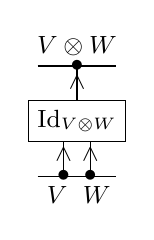
\begin{tikzpicture}[yscale = 0.7, baseline = 0pt]
\draw (0,0) -- (1,0) node[pos = 0.25,below]{\small $V$} node[pos = 0.33]{\small $\bullet$} node[pos = 0.67]{\small $\bullet$} node[pos = 0.75,below]{\small $W$};
\draw (0,2) -- (1,2) node[pos = 0.5]{\small $\bullet$} node[midway,above]{\small $V \otimes W$};
\draw (0.33,0) -- ++(0,1) node[pos = 0.4, sloped]{\footnotesize $>$};
\draw (0.67,0) -- ++(0,1) node[pos = 0.4, sloped]{\footnotesize $>$};
\draw (0.5,1) -- ++(0,1) node[pos = 0.7, sloped]{\footnotesize $>$};
\node[draw, rectangle, fill=white] at (0.5,1) {\small ${\rm Id}_{V \otimes W}$};
\end{tikzpicture}
$$
\end{Remark}

\begin{Remark}[{\cite[Remark 1.7]{Cooke}}]\label{Skmonoidal}
For a general surface $\Sigma$, the categories defined above are not monoidal because there is no notion of horizontal juxtaposition, which we used in $\mathbb{R}^2$. However, if $A = C \times [0,1]$ for a 1-manifold $C$, the category ${\rm Sk}_\mathcal{V}(A)$ is monoidal with tensor product induced by $A \sqcup A \overset{[0,\frac{1}{3}]\sqcup[\frac{2}{3},1]}\hookrightarrow A$.
\end{Remark}

\begin{Remark}[{\cite[Remarks 1.6 and 1.18]{Cooke}}]\label{rmkFunctEmbIsotOfSkCat} An orientation-preserving smooth embedding $f\colon\Sigma_1 \allowbreak\to \Sigma_2$ induces a functor ${\rm Sk}_\mathcal{V}(f)\colon{\rm Sk}_\mathcal{V}(\Sigma_1)\to {\rm Sk}_\mathcal{V}(\Sigma_2)$. It maps an object $s$, which is a bunch of coloured points in $\Sigma_1$, to $f(s)$, and a ribbon graph $T \subseteq \Sigma_1 \times [0,1]$ to $(f\times {\rm Id})(T)$. This defines a symmetric monoidal functor ${\rm Sk}_\mathcal{V}\colon ({\rm Mfld}_2^{\rm or},\sqcup) \to ({\rm Cat}_k,\otimes_k)$.

An isotopy of smooth embeddings $\lambda \colon \Sigma_1 \times [0,1] \to \Sigma_2$ between $f=\lambda_0$ and $g=\lambda_1$ induces a~natural isomorphism ${\rm rib}_\lambda\colon {\rm Sk}_\mathcal{V}(f) \Rightarrow {\rm Sk}_\mathcal{V}(g)$, where ${\rm rib}_{\lambda,s}\colon f(s) \to g(s)$ is the braid in $\Sigma_2 \times [0,1]$ drawn by $\{(\lambda_t(s),t), t \in [0,1]\}$. Homotopic isotopies give isotopic ribbon graphs, and this extends to a symmetric monoidal $\infty$-functor ${\rm Sk}_\mathcal{V}\colon ({\rm Mfld}_2^{\rm or},\sqcup) \to ({\rm Cat}_k,\otimes_k)$. It is shown in~\cite{Cooke} that this functor is the factorisation homology with coefficients in $\mathcal{V}$.
\end{Remark}

\begin{Proposition}[{\cite[Section~1.3]{Cooke}}]\label{Skmodcat}
For $C\subset \partial \Sigma$ a boundary component $($actually, a thick left boundary component, i.e., equipped with an embedding $C \times [0,2) \hookrightarrow \Sigma)$ the category ${\rm Sk}_\mathcal{V}(\Sigma)$ inherits a~structure of left ${\rm Sk}_\mathcal{V}(A)$-module category, where $A = C\times [0,1]$. Namely, one has a~functor $\rhd\colon {\rm Sk}_\mathcal{V}(A) \otimes {\rm Sk}_\mathcal{V}(\Sigma) \to {\rm Sk}_\mathcal{V}(\Sigma)$ compatible with the monoidal structure of ${\rm Sk}_\mathcal{V}(A)$. It is given by pushing points or ribbon graphs in $A$ inside $\Sigma$.
Similarly, a thick right boundary component $C\times (-1,1]\hookrightarrow \Sigma$ induces a right ${\rm Sk}_\mathcal{V}(A)$-module structure on ${\rm Sk}_\mathcal{V}(\Sigma)$.
\end{Proposition}

\setcounter{Theorem}{19}
% Original source lines 503--1071
\begin{Example}
We are particularly interested in the case $\mathcal{V} = \Oq\text{-}{\rm comod}^{\rm fin}$, for which the relations the Reshetikhin--Turaev functor imposes (between framed tangles) are precisely the Kauffman-bracket relations.
\end{Example}

\begin{Remark}\label{rmkUnorTanOq}
In any skein category, the identity coupon ${\rm Id}_{X^*}\colon X^* \to X^*$ with entry a downward oriented $X$-coloured ribbon and output an upward oriented $X^*$-coloured ribbon depicted below gives an identification $(X,-) \simeq (X^*,+)$.
$$
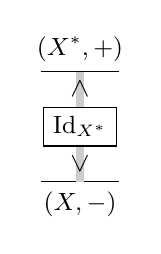
\begin{tikzpicture}[yscale = 0.7, baseline = 0pt]
\draw (0,0) -- (1,0) node[midway,below]{\small $(X,-)$};
\draw (0,2) -- (1,2) node[midway,above]{\small $(X^*,+)$};
\node[draw, rectangle] (I) at (0.5,1) {\small ${\rm Id}_{X^*}$};
\draw[gray!40, line width = 3pt] (0.5,0) -- (I) node[midway, sloped, black]{$<$} -- (0.5,2) node[midway, sloped, black]{$>$};
\end{tikzpicture}
$$
In the case $\mathcal{V} = \Oq\text{-}{\rm comod}^{\rm fin}$ and $X = V$ is the standard corepresentation, the object~$V^*$ is already isomorphic to $V$ in $\mathcal{V}$ by $\varphi$ from Definition~\ref{defOqcomods}. Thus one gets an identification $(V,+) \simeq (V,-)$ and sliding the coupon coloured by it along a strand changes the orientation of the strand. Consequently, one can switch signs of points and orientations of strands.
\end{Remark}

 In the following, we stop mentioning them and talk about unoriented framed tangles. The Reshetikin--Turaev functor is still well-defined on unoriented framed tangles, see \cite[Theorem~4.2]{Tingley}. An unoriented tangle gives a ribbon graph by choosing an arbitrary orientation, colouring every strand by $V$ and replacing $V^*$'s imposed on the boundary points by $V$'s using $\varphi$ or $\varphi^{-1}$. Concretely, for the unoriented cap $\cap$ for example, one can orient it either left or right, so one has to check that $\mathop{\rm RT}(\lcap) \circ (\varphi \otimes {\rm Id}_V) = \mathop{\rm RT}(\rcap) \circ ({\rm Id}_V \otimes \varphi)$. Note that this would not hold with the usual coribbon element in $\Oq$.

{\sloppy\begin{Theorem}[{\cite[Theorem~12.3.10]{CP}} or {\cite[Theorem~3.3.4]{Carter}} for endomorphisms in $\mathbb{R}^2$]\label{thmSkAsTangles}
Let~$n.V$ and~$m.V$ be two objects of ${\rm Sk}_\mathcal{V}(\Sigma)$ given respectively by $n$ and $m$ points coloured by $V$. Then any morphism in $\Hom_{{\rm Sk}_\mathcal{V}(\Sigma)}(n.V,m.V)$ can be represented by a linear combination of unoriented framed tangles $($without coupons$)$. Moreover, two linear combinations of unoriented framed tangles represent the same morphism in $\Hom_{{\rm Sk}_\mathcal{V}(\Sigma)}(n.V,m.V)$ if and only if one can get from one to the other by a~sequence of isotopies and Kauffman-bracket relations.
\end{Theorem}}

\begin{Corollary}
The algebra $\Hom_{{\rm Sk}_\mathcal{V}(\mathbb{R}^2)}(n.V,n.V)$ is isomorphic to the Temperley--Lieb algebra~${\rm TL}_n$, defined in {\rm \cite[Section~XII.3]{Turaev}}. The full subcategory of ${\rm Sk}_\mathcal{V}\big(\mathbb{R}^2\big)$ of objects of the form~$[n]$ with every point coloured by $V$ is equivalent to the category ${\rm TL}$, defined in {\rm\cite[Section~XII.2]{Turaev}}. In the following, we will call this full subcategory ${\rm TL}$.
\end{Corollary}

The category ${\rm TL}$ is a ribbon full subcategory of $\mathcal{V}$, and the above theorem proves that for any surface $\Sigma$ the category ${\rm Sk}_{{\rm TL}}(\Sigma)$ is a full subcategory of ${\rm Sk}_\mathcal{V}(\Sigma)$.

\subsection{Stated skein algebras}\label{SectStatedSkein} Stated skein algebras generalise skein algebras for tangles on a marked surface with boundary, see \cite{BonahonWong,TTQLe,Muller}. These tangles can be cut and stated skein algebras satisfy nice excision properties. We will recall here the approach of \cite{Cos}. Stated skein algebras can be defined over integral rings of coefficients, but we will work over a field $k$ being either $\mathbb{Q}\big(q^{\frac{1}{2}}\big)$ or $\mathbb{C}$ with $q^{\frac{1}{2}} \in \mathbb{C}^\times$ generic, as our proofs only hold in this context.

\begin{Definition}
Let $\mathfrak{S}$ be an oriented surface. The skein algebra $\mathring{\mathscr{S}}(\mathfrak{S})$ is the $k$-vector space generated by isotopy classes of unoriented framed links in $\mathfrak{S}\times (0,1)$ modulo the skein relations:
\[ \Kauftresse \ = q \Kaufvert\ +q^{-1} \Kaufhoriz \qquad \text{and} \qquad \Kaufcirc \ = \big({-}q^2-q^{-2}\big) \Kaufvide \]
in a little embedded cube $\phi\colon \mathbb{D}^3 \hookrightarrow \mathfrak{S}\times (0,1)$.

It is an algebra with product given by vertical superposition $\mathfrak{S}\times (0,1) \sqcup \mathfrak{S}\times (0,1) \overset{\left(\frac{1}{2},1\right)\sqcup\left(0,\frac{1}{2}\right)}\longrightarrow \mathfrak{S} \times (0,1)$ and unit the empty link.
\end{Definition}

Note that by Theorem~\ref{thmSkAsTangles}, one has an algebra isomorphism
\[
\mathring{\mathscr{S}}(\mathfrak{S}) \simeq \End_{{\rm Sk}_{\Oqcomfin}(\Sigma)}(\varnothing).
\]

\begin{Definition}
A marked surface is a compact oriented surface with boundary $\overline{\mathfrak{S}}$ with a finite set $P\subseteq \partial\overline{\mathfrak{S}}$ of boundary points, called marked points. We write $\mathfrak{S} = \overline{\mathfrak{S}} \smallsetminus P$ and call this the marked surface. We write $\partial_P\overline{\mathfrak{S}}$ the boundary components of $\overline{\mathfrak{S}}$ that contain a point of $P$ and $\partial \mathfrak{S} := \partial_P\overline{\mathfrak{S}} \smallsetminus P$. Namely we only consider boundary components of $\mathfrak{S}$ that contain a marked point, which we remove in $\mathfrak{S}$, so all components of $\partial \mathfrak{S}$ are intervals. The circular boundary components are discarded and give punctures in $\mathfrak{S}$. The boundary structure of stated skein algebras will depend on a way to cut out a bigon out of a~boundary edge, and that of internal skein algebras on a way to insert one from a~boundary edge. To avoid choices, we suppose that marked surfaces come equipped with a thickening of their boundary edges inside the surface.

A stated tangle $\alpha$ on $\mathfrak{S}$ is an unoriented, framed, compact, properly embedded 1-submanifold of $\mathfrak{S} \times (0,1)$ whose boundary $\partial \alpha \subseteq \partial\mathfrak{S} \times (0,1)$ has positively vertical framing and comes equipped with a~state ${\rm st}\colon \partial \alpha \to \{+,-\}$. We call height the $(0,1)$-coordinate of a point, and require that all boundary points of $\alpha$ lying over a same component of $\partial\mathfrak{S}$ have distinct heights. An isotopy of stated tangles is an isotopy with values in stated tangles, in particular preserving the height order over a same boundary component. A stated tangle in $\mathfrak{S} \times (0,1)$ can always be represented as a diagram with blackboard framing in $\mathfrak{S}$, with its under/over crossing information, such that the height order of boundary points corresponds to a given orientation on the boundary edges, see \cite[Section~3.5]{BonahonWong}.
\end{Definition}

\begin{Definition}[{\cite[Section~2.5]{Cos}}]
The stated skein algebra $\mathscr{S}(\mathfrak{S})$ of a marked surface $\mathfrak{S}$ is the $k$-vector space generated by isotopy classes of stated tangles on $\mathfrak{S}$ modulo usual skein relations:
\[
\Kauftresse \ = q \Kaufvert\ + q^{-1} \Kaufhoriz\,, \qquad
\Kaufcirc \ = \big({-}q^2-q^{-2}\big)\, \Kaufvide\
\]
and the boundary skein relations:
\[
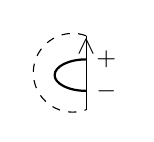
\begin{tikzpicture}[scale = 0.5, baseline = -3pt]
\draw[dashed] (70:1) arc(70:290:1);
\draw (-70:1) -- (70:1) node[pos = 0.85,sloped]{\small $>$};
\draw[thick] (70:1)++ (0,-0.6) node[right]{\small $+$} arc(90:270:0.8 and 0.4) node[right]{\small $-$};
\end{tikzpicture}
= q^{-\frac{1}{2}} \begin{tikzpicture}[scale = 0.5, baseline = -3pt]
\draw[dashed] (70:1) arc(70:290:1);
\draw (-70:1) -- (70:1) node[pos = 0.85,sloped]{\small $>$};
\end{tikzpicture}\!, \qquad
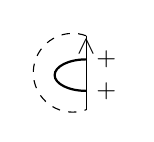
\begin{tikzpicture}[scale = 0.5, baseline = -3pt]
\draw[dashed] (70:1) arc(70:290:1);
\draw (-70:1) -- (70:1) node[pos = 0.85,sloped]{\small $>$};
\draw[thick] (70:1)++ (0,-0.6) node[right]{\small $+$} arc(90:270:0.8 and 0.4) node[right]{\small $+$};
\end{tikzpicture} = 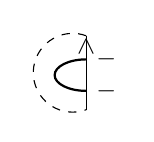
\begin{tikzpicture}[scale = 0.5, baseline = -3pt]
\draw[dashed] (70:1) arc(70:290:1);
\draw (-70:1) -- (70:1) node[pos = 0.85,sloped]{\small $>$};
\draw[thick] (70:1)++ (0,-0.6) node[right]{\small $-$} arc(90:270:0.8 and 0.4) node[right]{\small $-$};
\end{tikzpicture} = 0,
\qquad
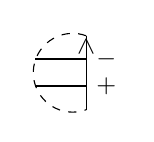
\begin{tikzpicture}[scale = 0.5, baseline = -3pt]
\draw[dashed] (70:1) arc(70:290:1);
\draw (-70:1) -- (70:1) node[pos = 0.85,sloped]{\small $>$};
\draw[thick] (70:1)++ (0,-0.6) node[right]{\small $-$} -- ++(-1.3,0);
\draw[thick] (-70:1)++ (0,0.6) node[right]{\small $+$} -- ++(-1.3,0);
\end{tikzpicture}
=q^2 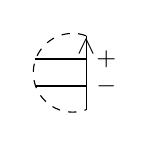
\begin{tikzpicture}[scale = 0.5, baseline = -3pt]
\draw[dashed] (70:1) arc(70:290:1);
\draw (-70:1) -- (70:1) node[pos = 0.85,sloped]{\small $>$};
\draw[thick] (70:1)++ (0,-0.6) node[right]{\small $+$} -- ++(-1.3,0);
\draw[thick] (-70:1)++ (0,0.6) node[right]{\small $-$} -- ++(-1.3,0);
\end{tikzpicture}
+q^{-\frac{1}{2}} 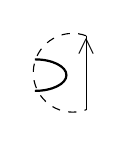
\begin{tikzpicture}[scale = 0.5, baseline = -3pt]
\draw[dashed] (70:1) arc(70:290:1);
\draw (-70:1) -- (70:1) node[pos = 0.85,sloped]{\small $>$};
\draw[thick] (70:1)++ (-1.3,-0.6) arc(90:-90:0.8 and 0.4);
\end{tikzpicture}\!,
\]
where the arrows on the boundary edges represent the relative height order of the two points.
It is an algebra with product given by vertical superposition and unit the empty link.

We denote by $C^\mu_\nu$ the coefficient such that
\[
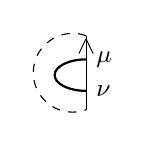
\begin{tikzpicture}[scale = 0.5, baseline = -3pt]
\draw[dashed] (70:1) arc(70:290:1);
\draw (-70:1) -- (70:1) node[pos = 0.85,sloped]{\small $>$};
\draw[thick] (70:1)++ (0,-0.6) node[right]{\small $\mu$} arc(90:270:0.8 and 0.4) node[right]{\small $\nu$};
\end{tikzpicture} = C^\mu_\nu \begin{tikzpicture}[scale = 0.5, baseline = -3pt]
\draw[dashed] (70:1) arc(70:290:1);
\draw (-70:1) -- (70:1) node[pos = 0.85,sloped]{\small $>$};
\end{tikzpicture},
\]
namely $C_+^+ = C_-^- = 0$, $C^+_-=q^{-\frac{1}{2}}$ and one can compute $C^-_+ = -q^{-\frac{5}{2}}$, see \cite[Lemma~2.3(13)]{Cos}. We~also write $C(\nu) := C_\nu^{-\nu}$.
\end{Definition}

\begin{Proposition}[{\cite[Lemmas 2.3 and 2.4]{TTQLe}}] \label{propLeftStSkRel}
These relations express equivalently with the boundary at the left, namely:
\[
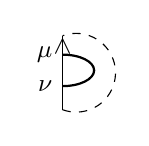
\begin{tikzpicture}[scale = 0.5, baseline = -3pt, rotate = 180]
\draw[dashed] (70:1) arc(70:290:1);
\draw (-70:1) -- (70:1) node[pos = 0.15,sloped]{\small $>$};
\draw[thick] (70:1)++ (0,-0.6) node[left]{\small $\nu$} arc(90:270:0.8 and 0.4) node[left]{\small $\mu$};
\end{tikzpicture} = {}^{\mu}_{\nu}\reflectbox{$C$} \begin{tikzpicture}[scale = 0.5, baseline = -3pt, rotate = 180]
\draw[dashed] (70:1) arc(70:290:1);
\draw (-70:1) -- (70:1) node[pos = 0.15,sloped]{\small $>$};
\end{tikzpicture},
\]
where ${}^+_+ \reflectbox{$C$} = {}^-_-\reflectbox{$C$}=0$, ${}^+_-\reflectbox{$C$}= -q^{\frac{5}{2}}$ and ${}^-_+\reflectbox{$C$}= q^{\frac{1}{2}}$, and
\[
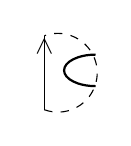
\begin{tikzpicture}[scale = 0.5, baseline = -3pt, rotate = 180]
\draw[dashed] (70:1) arc(70:290:1);
\draw (-70:1) -- (70:1) node[pos = 0.15,sloped]{\small $>$};
\draw[thick] (70:1)++ (-1.3,-0.6) arc(90:-90:0.8 and 0.4);
\end{tikzpicture} = q^{-\frac{1}{2}} 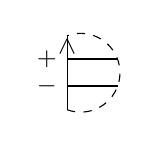
\begin{tikzpicture}[scale = 0.5, baseline = -3pt, rotate = 180]
\draw[dashed] (70:1) arc(70:290:1);
\draw (-70:1) -- (70:1) node[pos = 0.15,sloped]{\small $>$};
\draw[thick] (70:1)++ (0,-0.6) node[left]{\small $-$} -- ++(-1.3,0);
\draw[thick] (-70:1)++ (0,0.6) node[left]{\small $+$} -- ++(-1.3,0);
\end{tikzpicture} -q^{-\frac{5}{2}} 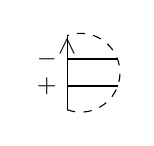
\begin{tikzpicture}[scale = 0.5, baseline = -3pt, rotate = 180]
\draw[dashed] (70:1) arc(70:290:1);
\draw (-70:1) -- (70:1) node[pos = 0.15,sloped]{\small $>$};
\draw[thick] (70:1)++ (0,-0.6) node[left]{\small $+$} -- ++(-1.3,0);
\draw[thick] (-70:1)++ (0,0.6) node[left]{\small $-$} -- ++(-1.3,0);
\end{tikzpicture}.
\]
\end{Proposition}

\begin{Remark}
It is easy to check that $\mathscr{S}(\mathfrak{S} \sqcup \mathfrak{S}') \simeq \mathscr{S}(\mathfrak{S}) \otimes_k \mathscr{S}(\mathfrak{S}')$ since all relations happen in a~connected disk.
\end{Remark}

\begin{Definition} [see {\cite[Section~3.1]{TTQLe}} for details]
Let $\mathfrak{S}$ be a marked surface and $c$ an ideal arc on~$\mathfrak{S}$, joining two marked points in $\overline{\mathfrak{S}}$. Denote by ${\rm Cut}_c(\mathfrak{S})$ the marked surface obtained by cutting $\mathfrak{S}$ along~$c$.

Given a stated tangle $\alpha$ on $\mathfrak{S}$, one can cut it along $c$ and get a tangle ${\rm Cut}_c(\alpha)$ on ${\rm Cut}_c(\mathfrak{S})$. This tangle has new boundary points, two lifts per points of $\alpha \cap c$, and we may give any state to these points. The obtained stated tangle is called a lift of $\alpha$ if the two lifts of a point of $\alpha \cap c$ have same state.
\end{Definition}

This definition is not perfectly innocent and it seems that one could have chosen different state-matching patterns for lifts, see Remark \ref{rmkChoiceCutting}.

\begin{Theorem}[{\cite[Theorem~3.1]{TTQLe}}]\label{splitmorph} Let $\mathfrak{S}$ be a marked surface and $c$ an ideal arc. The map $\rho_c\colon \mathscr{S}(\mathfrak{S}) \to \mathscr{S}({\rm Cut}_c(\mathfrak{S}))$, $\alpha \mapsto \sum_{\rm lifts} \tilde{\alpha}$ is well-defined $($it only depends on the isotopy class of~$\alpha)$ and is an injective algebra morphism. Moreover, the splitting morphisms $\rho_c$ and $\rho_{c'}$ associated to two disjoint ideal arcs $c$ and $c'$ commute.
\end{Theorem}

\begin{Example}
The bigon $B$ is the marked surface $(\mathbb{D},\{\pm i\})$, the disk with two marked points. The algebra $\mathscr{S}(B)$ is generated as an algebra by the
\[
{}_\mu\beta_\nu = 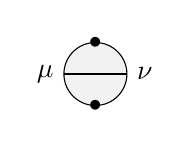
\begin{tikzpicture}[scale = 0.8, baseline = -5pt]
\fill [gray!10] (0,0) circle (0.5);
\draw (0,0) circle (0.5);
\node at (0,-0.5){\small $\bullet$};
\node at (0,0.5){\small $\bullet$};
\draw [thick] (-0.5,0) node[left]{$\mu$} -- (0.5,0) node[right]{$\nu$};
\end{tikzpicture}\!\!, \qquad
\mu,\nu \in \{\pm\},
\]
and has basis the
\[_{\vec{\mu}}\beta_{\vec{\nu}} = 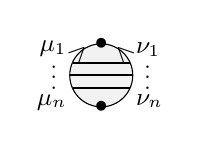
\begin{tikzpicture}[scale = 0.8, baseline = -5pt]
\fill [gray!10] (0,0) circle (0.5);
\draw (0,0) circle (0.5);
\node[rotate = 45] at (135:0.5) {\small $>$};
\node[rotate = -45] at (45:0.5) {\small $<$};
\node at (0,-0.5){\small $\bullet$};
\node at (0,0.5){\small $\bullet$};
\draw [thick] (-0.5,0) node[rotate = 90, above]{\footnotesize $\cdots$} -- (0.5,0) node[rotate = 90, below]{\footnotesize $\cdots$};
\draw [thick] (-0.45,-0.2) node[below left = -2pt]{\small $\mu_n$} -- (0.45,-0.2) node[below right = -2pt]{\small $\nu_n$};
\draw [thick] (-0.45,0.2) node[above left = -2pt]{\small $\mu_1$} -- (0.45,0.2) node[above right = -2pt]{\small $\nu_1$};
\end{tikzpicture}\!,
\]
where $\vec{\mu} = (\mu_1,\ldots,\mu_n)$ and $\vec{\nu} = (\nu_1,\ldots,\nu_n)$ are decreasing sequences of signs.

It is a bialgebra with coproduct given by cutting along the ``unique'' arc joining the two marked points \[
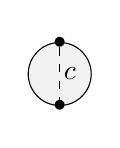
\begin{tikzpicture}[scale = 0.8, baseline = -5pt]
\fill [gray!10] (0,0) circle (0.5);
\draw (0,0) circle (0.5);
\node at (0,-0.5){\small $\bullet$};
\node at (0,0.5){\small $\bullet$};
\draw [dashed] (0,-0.5) -- (0,0.5) node[midway, right = -2pt]{$c$};
\end{tikzpicture}, \qquad
\Delta=\rho_c\colon\ \mathscr{S}(B) \to \mathscr{S}(B \sqcup B) \simeq \mathscr{S}(B) \otimes \mathscr{S}(B).
\]
Coassociativity comes from the second part of Theorem~\ref{splitmorph}. The counit $\varepsilon\colon \mathscr{S}(B) \to k$ is defined on the basis by $\varepsilon(_{\vec{\mu}}\beta_{\vec{\nu}}) = \delta_{\vec{\mu},\vec{\nu}}$.
It is a Hopf algebra with antipode
\[
S\Bigg(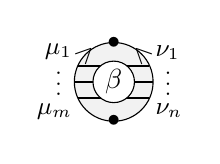
\begin{tikzpicture}[scale = 1, baseline = -5pt]
\fill [gray!10] (0,0) circle (0.5);
\draw (0,0) circle (0.5);
\node[rotate = 45] at (135:0.5) {\small $>$};
\node[rotate = -45] at (45:0.5) {\small $<$};
\node at (0,-0.5){\small $\bullet$};
\node at (0,0.5){\small $\bullet$};
\draw [thick] (-0.5,0) node[rotate = 90, above]{\footnotesize $\cdots$} -- (0.5,0) node[rotate = 90, below]{\footnotesize $\cdots$};
\draw [thick] (-0.45,-0.2) node[below left = -2pt]{\small $\mu_m$} -- (0.45,-0.2) node[below right = -2pt]{\small $\nu_n$};
\draw [thick] (-0.45,0.2) node[above left = -2pt]{\small $\mu_1$} -- (0.45,0.2) node[above right = -2pt]{\small $\nu_1$};
\node[circle, fill = white, draw = black, inner sep = 1.5pt] at (0,0) {$\beta$};
\end{tikzpicture}\!\!\Bigg)=
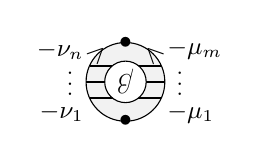
\begin{tikzpicture}[scale = 1, baseline = -5pt]
\fill [gray!10] (0,0) circle (0.5);
\draw (0,0) circle (0.5);
\node[rotate = 45] at (135:0.5) {\small $>$};
\node[rotate = -45] at (45:0.5) {\small $<$};
\node at (0,-0.5){\small $\bullet$};
\node at (0,0.5){\small $\bullet$};
\draw [thick] (-0.5,0) node[rotate = 90, above]{\footnotesize $\cdots$} -- (0.5,0) node[rotate = 90, below]{\footnotesize $\cdots$};
\draw [thick] (-0.45,-0.2) node[below left = -2pt]{\small $-\nu_1$} -- (0.45,-0.2) node[below right = -2pt]{\small $-\mu_1$};
\draw [thick] (-0.45,0.2) node[above left = -2pt]{\small $-\nu_n$} -- (0.45,0.2) node[above right = -2pt]{\small $-\mu_m$};
\node[circle, rotate = 180, fill = white, draw = black, inner sep = 1.5pt] at (0,0) {$\beta$};
\end{tikzpicture}
 .\ \frac{C(\vec{\nu})}{C(\vec{\mu})},\qquad
\text{where}\qquad C(\vec{\nu}):= \prod_{i=1}^n C(\nu_i).
 \]
It is coquasitriangular with co-$R$-matrix
\[
R(\alpha \otimes \beta) =\varepsilon
\raisebox{0pt}{$\left(\rule{-3pt}{22pt}\right.$}\!
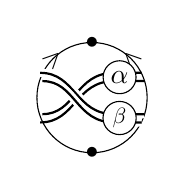
\begin{tikzpicture}[scale = 0.7, baseline = 0pt, rotate = 180]
\draw (0,-1) node{\small $\bullet$} arc(-90:90:1) node[near start, sloped]{\small $>$} node{\small $\bullet$};
\draw (0,-1) arc(-90:-270:1) node[near start, sloped]{\small $<$};
\draw[thick] (-0.9,-0.45) -- (-0.4,-0.45) .. controls (0.3,-0.45) and (0.3,0.3).. (0.9,0.3);
\draw[thick] (-0.94,-0.3) -- (-0.4,-0.3) .. controls (0.3,-0.3) and (0.3,0.45).. (0.94,0.45);
\draw[line width = 3pt, white] (-0.94,0.3) -- (-0.4,0.3) .. controls (0.3,0.3) and (0.3,-0.45).. (0.94,-0.45);
\draw[thick] (-0.94,0.3) -- (-0.4,0.3) .. controls (0.3,0.3) and (0.3,-0.45).. (0.94,-0.45);
\draw[line width = 3pt, white] (-0.9,0.45) -- (-0.4,0.45) .. controls (0.3,0.45) and (0.3,-0.3).. (0.9,-0.3);
\draw[thick] (-0.9,0.45) -- (-0.4,0.45) .. controls (0.3,0.45) and (0.3,-0.3).. (0.9,-0.3);
\node[circle, fill=white, draw = black, scale = 0.8, inner sep = 1.5pt] (X) at (-0.5,0.37){$\beta$};
\node[circle, fill=white, draw = black, scale = 1, inner sep = 1.5pt] (X) at (-0.5,-0.37){$\alpha$};
\end{tikzpicture}\!
\raisebox{0pt}{$\left.\rule{-3pt}{22pt}\right)$}\!,
\]
see \cite[Theorem~3.5]{Cos}.
It is coribbon with coribbon functional
\[
\theta(\alpha) = \varepsilon
\raisebox{0pt}{$\left(\rule{-3pt}{22pt}\right.$}\!
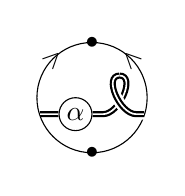
\begin{tikzpicture}[scale = 0.7, baseline = 0pt]
\draw (0,-1) node{\small $\bullet$} arc(-90:90:1) node[near end, sloped]{\small $<$} node{\small $\bullet$};
\draw (0,-1) arc(-90:-270:1) node[near end, sloped]{\small $>$};
\node[circle, draw = black, scale = 1, inner sep = 1.5pt] (X) at (-0.3,-0.3){$\alpha$};
\draw[thick, double] (-0.94,-0.3) -- (X) -- (0.2,-0.3) .. controls (0.5,-0.3) and (0.8,0.4).. (0.5,0.4);
\draw[line width = 4pt, white] (0.5,0.4).. controls (0.2,0.4) and (0.5,-0.3) .. (0.8,-0.3) -- (0.94,-0.3);
\draw[thick, double] (0.5,0.4).. controls (0.2,0.4) and (0.5,-0.3) .. (0.8,-0.3) -- (0.94,-0.3);
\end{tikzpicture}\!
\raisebox{0pt}{$\left.\rule{-3pt}{22pt}\right)$}\!.
\]
\end{Example}

\begin{Proposition}[{\cite[Theorem~4.1]{TTQLe}, \cite[Section~2.2]{KorQue}}, {\cite[Theorem~3.4]{Cos}}]
One has an isomorphism of coribbon Hopf algebras $\mathscr{S}(B)\simeq \Oq$ given on the generators by $_+\beta_+\mapsto a$, ${}_-\beta_{-}\mapsto d$,  ${}_+\beta_{-}\mapsto b$ and ${}_-\beta_{+}\mapsto c$.
\end{Proposition}
Stated skein algebras provide great examples of (possibly infinite-dimensional) $\Oq$ or $\mathscr{S}(B)$-comodules.

Given a marked surface $\mathfrak{S}$ and a boundary edge $e$ of $\mathfrak{S}$, we can consider an ideal arc $c$ going along~$e$ but inside $\mathring{\mathfrak{S}}$. The piece between $e$ and $c$ is a bigon, and the rest is homeomorphic to the original surface. The splitting morphism along $c$, $\Delta = \rho_c\colon \mathscr{S}(\mathfrak{S}) \to \mathscr{S}(\mathfrak{S}\sqcup B)\simeq \mathscr{S}(\mathfrak{S})\otimes \mathscr{S}(B)$ endows $\mathscr{S}(\mathfrak{S})$ with right $\Oq$-comodule structure.
$$
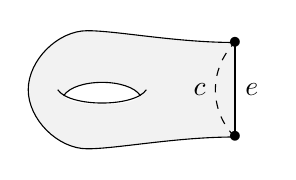
\begin{tikzpicture}[xscale = 0.75, yscale = 0.75,baseline = 10pt]
\fill[gray!10] (3.5,0.2) coordinate (B)	.. controls (2.5,0.2) and (1.5,0 ) .. (1,0)	.. controls (0.5,0 ) and (0,0.5 ) .. (0,1)	.. controls (0,1.5 ) and (0.5,2 ) .. (1,2)	.. controls (1.5,2 ) and (2.5,1.8) .. (3.5,1.8) coordinate (H) -- cycle ;
\fill[white] (0.6,0.9) .. controls (0.7,0.7) and (1.8,0.7) .. (1.9,0.9) .. controls (1.7,1.2) and (0.8,1.2) .. (0.6,0.9);
\draw (0.5,1) .. controls (0.7,0.7) and (1.8,0.7) .. (2,1);
\draw (0.6,0.9) .. controls (0.8,1.2) and (1.7,1.2) .. (1.9,0.9);
\draw (3.5,0.2) node{\small $\bullet$}	.. controls (2.5,0.2) and (1.5,0 ) .. (1,0)	.. controls (0.5,0 ) and (0,0.5 ) .. (0,1)	.. controls (0,1.5 ) and (0.5,2 ) .. (1,2)	.. controls (1.5,2 ) and (2.5,1.8) .. (3.5,1.8) node{\small $\bullet$};
\draw[thick] (B) -- (H) node[midway,right]{$e$};
\path[dashed, bend left = 150pt, in = 135, out = 45] (B) edge node[midway,left]{$c$} (H);
\end{tikzpicture}
$$
It is compatible with its algebra structure, namely $\mathscr{S}(\mathfrak{S})$ is an $\Oq$-comodule-algebra, see \cite[Proposition~4.1]{Cos}.

\begin{Definition}
Let $\operatorname{rot}\colon B \to B$ be the homeomorphism of marked surfaces given by the planar 180 degree rotation. It induces $\operatorname{rot}_*\colon \mathscr{S}(B) \to \mathscr{S}(B)$, with
\[
\operatorname{rot}_*\Bigg(
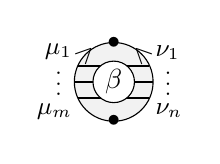
\begin{tikzpicture}[scale = 1, baseline = -5pt]
\fill [gray!10] (0,0) circle (0.5);
\draw (0,0) circle (0.5);
\node[rotate = 45] at (135:0.5) {\small $>$};
\node[rotate = -45] at (45:0.5) {\small $<$};
\node at (0,-0.5){\small $\bullet$};
\node at (0,0.5){\small $\bullet$};
\draw [thick] (-0.5,0) node[rotate = 90, above]{\footnotesize $\cdots$} -- (0.5,0) node[rotate = 90, below]{\footnotesize $\cdots$};
\draw [thick] (-0.45,-0.2) node[below left = -2pt]{\small $\mu_m$} -- (0.45,-0.2) node[below right = -2pt]{\small $\nu_n$};
\draw [thick] (-0.45,0.2) node[above left = -2pt]{\small $\mu_1$} -- (0.45,0.2) node[above right = -2pt]{\small $\nu_1$};
\node[circle, fill = white, draw = black, inner sep = 1.5pt] at (0,0) {$\beta$};
\end{tikzpicture}
\Bigg) =
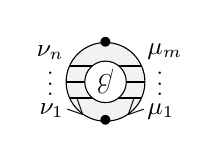
\begin{tikzpicture}[scale = 1, baseline = -5pt]
\fill [gray!10] (0,0) circle (0.5);
\draw (0,0) circle (0.5);
\node[rotate = 135] at (-135:0.5) {\small $<$};
\node[rotate = -135] at (-45:0.5) {\small $>$};
\node at (0,-0.5){\small $\bullet$};
\node at (0,0.5){\small $\bullet$};
\draw [thick] (-0.5,0) node[rotate = 90, above]{\footnotesize $\cdots$} -- (0.5,0) node[rotate = 90, below]{\footnotesize $\cdots$};
\draw [thick] (-0.45,-0.2) node[below left = -2pt]{\small $\nu_1$} -- (0.45,-0.2) node[below right = -2pt]{\small $\mu_1$};
\draw [thick] (-0.45,0.2) node[above left = -2pt]{\small $\nu_n$} -- (0.45,0.2) node[above right = -2pt]{\small $\mu_m$};
\node[circle, rotate = 180, fill = white, draw = black, inner sep = 1.5pt] at (0,0) {$\beta$};
\end{tikzpicture}
\]
which is an algebra isomorphism. It reverses the coproduct, namely
\[
\Delta\circ \operatorname{rot}_*(\beta) =
 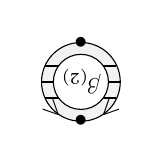
\begin{tikzpicture}[scale = 1, baseline = -5pt]
\fill [gray!10] (0,0) circle (0.5);
\draw (0,0) circle (0.5);
\node[rotate = 135] at (-135:0.5) {\small $<$};
\node[rotate = -135] at (-45:0.5) {\small $>$};
\node at (0,-0.5){\small $\bullet$};
\node at (0,0.5){\small $\bullet$};
\draw [thick] (-0.5,0) -- (0.5,0);
\draw [thick] (-0.45,-0.2) -- (0.45,-0.2) ;
\draw [thick] (-0.45,0.2) -- (0.45,0.2);
\node[circle, rotate = 180, fill = white, draw = black, inner sep = 1pt] at (0,0) {\footnotesize $\beta_{(2)}$};
\end{tikzpicture} \otimes 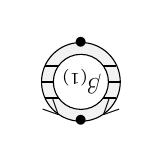
\begin{tikzpicture}[scale = 1, baseline = -5pt]
\fill [gray!10] (0,0) circle (0.5);
\draw (0,0) circle (0.5);
\node[rotate = 135] at (-135:0.5) {\small $<$};
\node[rotate = -135] at (-45:0.5) {\small $>$};
\node at (0,-0.5){\small $\bullet$};
\node at (0,0.5){\small $\bullet$};
\draw [thick] (-0.5,0) -- (0.5,0);
\draw [thick] (-0.45,-0.2) -- (0.45,-0.2) ;
\draw [thick] (-0.45,0.2) -- (0.45,0.2);
\node[circle, rotate = 180, fill = white, draw = black, inner sep = 1pt] at (0,0) {\footnotesize $\beta_{(1)}$};
\end{tikzpicture} = (\operatorname{rot}_*\otimes \operatorname{rot}_*) \circ \Delta^{\rm op} (\beta),
\]
and preserves the counit, because $\varepsilon(\operatorname{rot}_*(_{\vec{\mu}}\beta_{\vec{\nu}})) = \varepsilon(_{\vec{\nu}}\beta_{\vec{\mu}}) = \delta_{\vec{\nu},\vec{\mu}} = \delta_{\vec{\mu},\vec{\nu}}$.
On $\Oq$, it is given by $r\left(\begin{smallmatrix}a&b\\c&d\end{smallmatrix}\right) = \left( \begin{smallmatrix}a&c\\b&d\end{smallmatrix}\right)$.
\end{Definition}

\begin{Remark}If one sees the edge $e$ at the left instead of the right of the surface, one gets a~structure of left $\Oq$-comodule. One can easily get from one to another by rotating the whole picture. Namely, the left coaction $\Delta_{\rm l}$ is obtained from the right coaction $\Delta_{\rm r}$ by rotating the bigon by 180 degrees. In \cite[Proposition~4.1]{Cos} one gets $\Delta_{\rm l} = \operatorname{fl} \circ ({\rm Id}_{\mathscr{S}(\mathfrak{S})} \otimes \operatorname{rot}_*) \circ \Delta_{\rm r}$, where $\operatorname{fl}$ denotes the flip of tensors.
$$
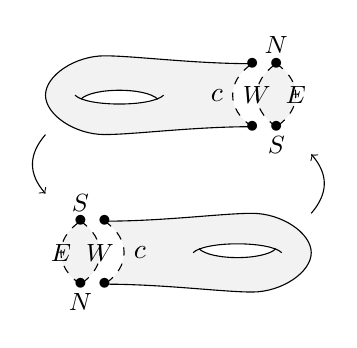
\begin{tikzpicture}[xscale = 0.75, yscale = 0.5,baseline = 10pt]
\fill[gray!10] (3.5,0.2) coordinate (B)	.. controls (2.5,0.2) and (1.5,0 ) .. (1,0)	.. controls (0.5,0 ) and (0,0.5 ) .. (0,1)	.. controls (0,1.5 ) and (0.5,2 ) .. (1,2)	.. controls (1.5,2 ) and (2.5,1.8) .. (3.5,1.8) coordinate (H) to[bend right = 150pt, in = -135, out = -45] (B) ;
\fill[white] (0.6,0.9) .. controls (0.7,0.7) and (1.8,0.7) .. (1.9,0.9) .. controls (1.7,1.2) and (0.8,1.2) .. (0.6,0.9);
\draw (0.5,1) .. controls (0.7,0.7) and (1.8,0.7) .. (2,1);
\draw (0.6,0.9) .. controls (0.8,1.2) and (1.7,1.2) .. (1.9,0.9);
\draw (3.5,0.2)node{\small $\bullet$}	.. controls (2.5,0.2) and (1.5,0 ) .. (1,0)	.. controls (0.5,0 ) and (0,0.5 ) .. (0,1)	.. controls (0,1.5 ) and (0.5,2 ) .. (1,2)	.. controls (1.5,2 ) and (2.5,1.8) .. (3.5,1.8) node{\small $\bullet$};
\path[dashed, bend left = 150pt, in = 135, out = 45] (B) edge node[midway,left]{$c$} (H);
\node [right= 8pt of B, inner sep = 0pt] (B') {};
\node [right= 8pt of H, inner sep = 0pt] (H') {};
\fill[gray!10] (B'.center)to[bend left = 150pt, in = 135, out = 45] (H'.center) to[bend left = 150pt, in = 135, out = 45] (B');
\draw[dashed] (B'.center) to[bend left = 150pt, in = 135, out = 45] node[pos = 0]{\small $\bullet$} node[pos = 1]{\small $\bullet$} node[midway]{\small $W$} (H'.center);
\draw[dashed] (H'.center) to[bend left = 150pt, in = 135, out = 45] node[midway]{\small $E$} node[pos = 1,below]{\small $S$} node[pos = 0,above]{\small $N$} (B'.center);
\draw[->] (0,0) to[bend right] ++(0,-1.5);
\begin{scope}[xshift = 4.5cm, yshift = -2cm, rotate = 180]
\fill[gray!10] (3.5,0.2) coordinate (B)	.. controls (2.5,0.2) and (1.5,0 ) .. (1,0)	.. controls (0.5,0 ) and (0,0.5 ) .. (0,1)	.. controls (0,1.5 ) and (0.5,2 ) .. (1,2)	.. controls (1.5,2 ) and (2.5,1.8) .. (3.5,1.8) coordinate (H) to[bend right = 150pt, in = -135, out = -45] (B) ;
\fill[white] (0.6,0.9) .. controls (0.7,0.7) and (1.8,0.7) .. (1.9,0.9) .. controls (1.7,1.2) and (0.8,1.2) .. (0.6,0.9);
\draw (0.5,1) .. controls (0.7,0.7) and (1.8,0.7) .. (2,1);
\draw (0.6,0.9) .. controls (0.8,1.2) and (1.7,1.2) .. (1.9,0.9);
\draw (3.5,0.2)node{\small $\bullet$}	.. controls (2.5,0.2) and (1.5,0 ) .. (1,0)	.. controls (0.5,0 ) and (0,0.5 ) .. (0,1)	.. controls (0,1.5 ) and (0.5,2 ) .. (1,2)	.. controls (1.5,2 ) and (2.5,1.8) .. (3.5,1.8) node{\small $\bullet$};
\path[dashed, bend left = 150pt, in = 135, out = 45] (B) edge node[midway,right]{$c$} (H);
\node [left= 8pt of B, inner sep = 0pt] (B') {};
\node [left= 8pt of H, inner sep = 0pt] (H') {};
\fill[gray!10] (B'.center)to[bend left = 150pt, in = 135, out = 45] (H'.center) to[bend left = 150pt, in = 135, out = 45] (B');
\draw[dashed] (B'.center) to[bend left = 150pt, in = 135, out = 45] node[pos = 0]{\small $\bullet$} node[pos = 1]{\small $\bullet$} node[midway]{\small $W$} (H'.center);
\draw[dashed] (H'.center) to[bend left = 150pt, in = 135, out = 45] node[midway]{\small $E$} node[pos = 1,above]{\small $S$} node[pos = 0,below]{\small $N$} (B'.center);
\draw[->] (0,0) to[bend right] ++(0,-1.5);
\end{scope}
\end{tikzpicture}
$$
Actually, one gets such a structure for each boundary edge of $\mathfrak{S}$, and if $\mathfrak{S}$ has $n$ right boundary edges and $m$ left, $\mathscr{S}(\mathfrak{S})$ is an $\big(\Oq^{\otimes n},\Oq^{\otimes m}\big)$-bicomodule algebra.
\end{Remark}

\begin{Remark}\label{rmkFormActOnSS}
The structure forms on $\mathscr{S}(B)$, such as the co-$R$-matrix or the coribbon functional, are often defined using the counit on some transformation of the tangle. This has a direct interpretation on how this form then acts on comodules.

Let $\varphi\colon\mathscr{S}(B) \to k$ be given by some
\[
\varphi\raisebox{-3pt}{$\left(\rule{0pt}{22pt}\right.$}\!\!
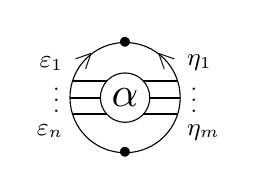
\begin{tikzpicture}[scale = 0.7, baseline = 0pt]
\draw (0,-1) node{\small $\bullet$} arc(-90:90:1) node[near end, sloped]{\small $<$} node{\small $\bullet$};
\draw (0,-1) arc(-90:-270:1) node[near end, sloped]{\small $>$};
\draw[thick] (-0.94,-0.3)node[below left]{\small $\varepsilon_n$} -- (0.94,-0.3)node[below right]{\small $\eta_m$};
\draw[thick] (-1,0) node[yshift=2pt,left]{\footnotesize $\vdots$} -- (1,0)node[yshift=2pt,right]{\footnotesize $\vdots$};
\draw[thick] (-0.94,0.3) node[above left]{\small $\varepsilon_1$} -- (0.94,0.3)node[above right]{\small $\eta_1$};
\node[circle, fill=white, draw = black, scale = 1.5, inner sep = 1.5pt] (X) at (0,0){$\alpha$};
\end{tikzpicture}\!\!
\raisebox{-3pt}{$\left.\rule{0pt}{22pt}\right)$}
 = \varepsilon
\raisebox{-3pt}{$\left(\rule{0pt}{32pt}\right.$}\!\!\!
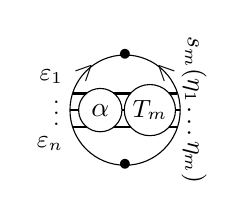
\begin{tikzpicture}[scale = 0.7, baseline = 0pt]
\draw (0,-1) node{\small $\bullet$} arc(-90:90:1) node[near end, sloped]{\small $<$} node{\small $\bullet$};
\draw (0,-1) arc(-90:-270:1) node[near end, sloped]{\small $>$};
\draw[thick] (-0.94,-0.3)node[below left]{\small $\varepsilon_n$} -- (0.94,-0.3);
\draw[thick] (-1,0) node[yshift=2pt,left]{\footnotesize $\vdots$} -- (1,0)node[xshift = 5pt, yshift = 0pt, rotate = -90]{\small $s_m(\eta_1 \dots \eta_m)$};
\draw[thick] (-0.94,0.3) node[above left]{\small $\varepsilon_1$} -- (0.94,0.3);
\node[circle, minimum width=0.55cm, fill=white, draw = black, scale = 1, inner sep = 1.5pt] (X) at (-0.45,0){$\alpha$};
\node[circle, minimum width=0.5cm,fill=white, draw = black, scale = 1, inner sep = 1.5pt] at (0.45,0){\small $T_m$};
\end{tikzpicture}\!
\raisebox{-3pt}{$\left.\rule{0pt}{32pt}\right)$},
\]
where $T_m,\ m \in \mathbb{N},$ is a family of tangles with $m$ right and $m$ left boundary points and $s_m\colon \{\pm\}^m\to {\rm vect}_ k(\{\pm\}^m)$. Here, we allowed $s_m$ to have values in formal linear combination of $m$-tuples of states because in the definition of the co-$R$-matrix for example one needs coefficients depending on the states. What we mean by a tangle $\alpha$ with state a formal linear combination of states $\sum_i \lambda_i \vec{\eta}_i$ is the linear sum of stated tangles $\alpha_{\sum_i \lambda_i \vec{\eta}_i} := \sum_i \lambda_i \alpha_{\vec{\eta}_i}$.
Note that the $T_m$'s and the $s_m$'s should satisfy extra conditions for this to be well-defined on $\mathscr{S}(B)$. Then for a marked surface $\mathfrak{S}$ with a right edge $e$, the map $\Phi_{\mathscr{S}(\mathfrak{S})}\colon \mathscr{S}(\mathfrak{S}) \overset{\Delta}{\to} \mathscr{S}(\mathfrak{S}) \otimes \mathscr{S}(B) \overset{{\rm Id} \otimes \varphi}{\longrightarrow} \mathscr{S}(\mathfrak{S})$ is given by
\[
\begin{array}{ll}
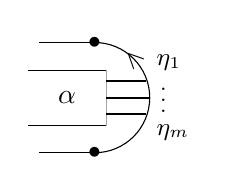
\begin{tikzpicture}[scale = 0.7, baseline = 0pt]
\draw (0,-1) node{\small $\bullet$} arc(-90:90:1) node[near end, sloped]{\small $<$} node{\small $\bullet$};
\draw (0,-1) -- (-1,-1);
\draw (0,1) -- (-1,1);
\draw[thick] (-1,-0.3) -- (0.94,-0.3)node[below right]{\small $\eta_m$};
\draw[thick] (-1,0) -- (1,0)node[yshift=2pt,right]{\footnotesize $\vdots$};
\draw[thick] (-1,0.3) -- (0.94,0.3)node[above right]{\small $\eta_1$};
\node[fill=white, minimum width = 1cm, minimum height = 0.7cm, leftymissy, inner sep = 1.5pt] (X) at (-0.5,0){$\alpha$};
\end{tikzpicture}
&\overset{\Delta}{\longmapsto} \sum_{\vec{\nu}}
\raisebox{-3pt}{$\left(\rule{0pt}{26pt}\right.$}
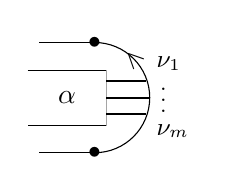
\begin{tikzpicture}[scale = 0.7, baseline = 0pt]
\draw (0,-1) node{\small $\bullet$} arc(-90:90:1) node[near end, sloped]{\small $<$} node{\small $\bullet$};
\draw (0,-1) -- (-1,-1);
\draw (0,1) -- (-1,1);
\draw[thick] (-1,-0.3) -- (0.94,-0.3)node[below right]{\small $\nu_m$};
\draw[thick] (-1,0) -- (1,0)node[yshift=2pt,right]{\footnotesize $\vdots$};
\draw[thick] (-1,0.3) -- (0.94,0.3)node[above right]{\small $\nu_1$};
\node[fill=white, minimum width = 1cm, minimum height = 0.7cm, leftymissy, inner sep = 1.5pt] (X) at (-0.5,0){$\alpha$};
\end{tikzpicture} \otimes
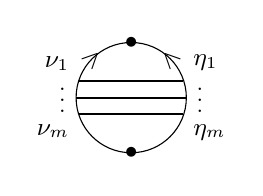
\begin{tikzpicture}[scale = 0.7, baseline = 0pt]
\draw (0,-1) node{\small $\bullet$} arc(-90:90:1) node[near end, sloped]{\small $<$} node{\small $\bullet$};
\draw (0,-1) arc(-90:-270:1) node[near end, sloped]{\small $>$};
\draw[thick] (-0.94,-0.3)node[below left]{\small $\nu_m$} -- (0.94,-0.3)node[below right]{\small $\eta_m$};
\draw[thick] (-1,0) node[yshift=2pt,left]{\footnotesize $\vdots$} -- (1,0)node[yshift=2pt,right]{\footnotesize $\vdots$};
\draw[thick] (-0.94,0.3) node[above left]{\small $\nu_1$} -- (0.94,0.3)node[above right]{\small $\eta_1$};
\end{tikzpicture}\!\!\!
\raisebox{-3pt}{$\left.\rule{0pt}{26pt}\right)$}
\\
& \overset{{\rm Id}\otimes \varphi}{\longmapsto} ({\rm Id} \otimes \varepsilon)
\raisebox{-3pt}{$\left(\rule{0pt}{32pt}\right.$}
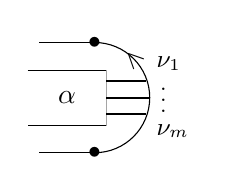
\begin{tikzpicture}[scale = 0.7, baseline = 0pt]
\draw (0,-1) node{\small $\bullet$} arc(-90:90:1) node[near end, sloped]{\small $<$} node{\small $\bullet$};
\draw (0,-1) -- (-1,-1);
\draw (0,1) -- (-1,1);
\draw[thick] (-1,-0.3) -- (0.94,-0.3)node[below right]{\small $\nu_m$};
\draw[thick] (-1,0) -- (1,0)node[yshift=2pt,right]{\footnotesize $\vdots$};
\draw[thick] (-1,0.3) -- (0.94,0.3)node[above right]{\small $\nu_1$};
\node[fill=white, minimum width = 1cm, minimum height = 0.7cm, leftymissy, inner sep = 1.5pt] (X) at (-0.5,0){$\alpha$};
\end{tikzpicture} \otimes
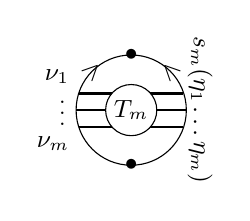
\begin{tikzpicture}[scale = 0.7, baseline = 0pt]
\draw (0,-1) node{\small $\bullet$} arc(-90:90:1) node[near end, sloped]{\small $<$} node{\small $\bullet$};
\draw (0,-1) arc(-90:-270:1) node[near end, sloped]{\small $>$};
\draw[thick] (-0.94,-0.3)node[below left]{\small $\nu_m$} -- (0.94,-0.3);
\draw[thick] (-1,0) node[yshift=2pt,left]{\footnotesize $\vdots$} -- (1,0)node[xshift = 5pt, yshift = 0pt, rotate = -90]{\small $s_m(\eta_1 \dots \eta_m)$};
\draw[thick] (-0.94,0.3) node[above left]{\small $\nu_1$} -- (0.94,0.3);
\node[circle, minimum width=0.5cm,fill=white, draw = black, scale = 1, inner sep = 1.5pt] at (0,0){\small $T_m$};
\end{tikzpicture}
\raisebox{-3pt}{$\left.\rule{0pt}{32pt}\right)$}
\\
& \overset{\rm splitting}{\underset{\rm well\ def}{=}} ({\rm Id} \otimes \varepsilon)
\raisebox{-3pt}{$\left(\rule{0pt}{32pt}\right.$}
\begin{tikzpicture}[scale = 0.7, baseline = 0pt]
\draw (0,-1) node{\small $\bullet$} arc(-90:90:1) node[near end, sloped]{\small $<$} node{\small $\bullet$};
\draw (0,-1) -- (-1,-1);
\draw (0,1) -- (-1,1);
\draw[thick] (-1,-0.3) -- (0.94,-0.3)node[below right]{\small $\nu_m$};
\draw[thick] (-1,0) -- (1,0)node[yshift=2pt,right]{\footnotesize $\vdots$};
\draw[thick] (-1,0.3) -- (0.94,0.3)node[above right]{\small $\nu_1$};
\node[fill=white, minimum width = 0.7cm, minimum height = 0.7cm, leftymissy, inner sep = 1.5pt] (X) at (-0.65,0){$\alpha$};
\node[circle, minimum width=0.5cm,fill=white, draw = black, scale = 1, inner sep = 1.5pt] at (0.4,0){\small $T_m$};
\end{tikzpicture} \otimes
\begin{tikzpicture}[scale = 0.7, baseline = 0pt]
\draw (0,-1) node{\small $\bullet$} arc(-90:90:1) node[near end, sloped]{\small $<$} node{\small $\bullet$};
\draw (0,-1) arc(-90:-270:1) node[near end, sloped]{\small $>$};
\draw[thick] (-0.94,-0.3)node[below left]{\small $\nu_m$} -- (0.94,-0.3);
\draw[thick] (-1,0) node[yshift=2pt,left]{\footnotesize $\vdots$} -- (1,0)node[xshift = 5pt, yshift = 0pt, rotate = -90]{\small $s_m(\eta_1 \dots \eta_m)$};
\draw[thick] (-0.94,0.3) node[above left]{\small $\nu_1$} -- (0.94,0.3);
\end{tikzpicture}
\raisebox{-3pt}{$\left.\rule{0pt}{32pt}\right)$}
\overset{\rm counit}{=}
\begin{tikzpicture}[scale = 0.7, baseline = 0pt]
\draw (0,-1) node{\small $\bullet$} arc(-90:90:1) node[near end, sloped]{\small $<$} node{\small $\bullet$};
\draw (0,-1) -- (-1,-1);
\draw (0,1) -- (-1,1);
\draw[thick] (-1,-0.3) -- (0.94,-0.3);
\draw[thick] (-1,0) -- (1,0)node[xshift = 5pt, yshift = 0pt, rotate = -90]{\small $s_m(\eta_1 \dots \eta_m)$};
\draw[thick] (-1,0.3) -- (0.94,0.3);
\node[fill=white, minimum width = 0.7cm, minimum height = 0.7cm, leftymissy, inner sep = 1.5pt] (X) at (-0.65,0){$\alpha$};
\node[circle, minimum width=0.5cm,fill=white, draw = black, scale = 1, inner sep = 1.5pt] at (0.4,0){\small $T_m$};
\end{tikzpicture}.
\end{array}
\]
The co-$R$-matrix isn't exactly of this form, but the same kind of computation applies. Remember that the braiding on $\mathscr{S}(\mathfrak{S}) \otimes \mathscr{S}(\mathfrak{S})$ is defined using the coaction on each $\mathscr{S}(\mathfrak{S})$, the co-$R$-matrix on the $\mathscr{S}(B)^{\otimes 2}$ part thus obtained, and then flipping the two factors, namely $c_{\mathscr{S}(\mathfrak{S}),\mathscr{S}(\mathfrak{S})} = \operatorname{fl} \circ R_{24}\circ \big(\Delta_{\mathscr{S}(\mathfrak{S})}\otimes \Delta_{\mathscr{S}(\mathfrak{S})}\big)$. The braided opposite product on $\mathscr{S}(\mathfrak{S})$ is defined as $m^{\rm bop} := m \circ c_{\mathscr{S}(\mathfrak{S}),\mathscr{S}(\mathfrak{S})}$ and it has a nice geometric depiction, namely:
\[
\begin{array}{ll}
m^{\rm bop}(\alpha \otimes \beta) & = m \circ \operatorname{fl}
\raisebox{-3pt}{$\left(\rule{0pt}{26pt}\right.$}
\begin{tikzpicture}[scale = 0.7, baseline = 0pt]
\draw (0,-1) node{\small $\bullet$} arc(-90:90:1) node[near end, sloped]{\small $<$} node{\small $\bullet$};
\draw (0,-1) -- (-1,-1);
\draw (0,1) -- (-1,1);
\draw[thick] (-1,-0.3) -- (0.94,-0.3)node[below right]{\small $\nu_n$};
\draw[thick] (-1,0) -- (1,0)node[yshift=2pt,right]{\footnotesize $\vdots$};
\draw[thick] (-1,0.3) -- (0.94,0.3)node[above right]{\small $\nu_1$};
\node[fill=white, minimum width = 1cm, minimum height = 0.7cm, leftymissy, inner sep = 1.5pt] (X) at (-0.5,0){$\alpha_{(1)}$};
\end{tikzpicture} \otimes \begin{tikzpicture}[scale = 0.7, baseline = 0pt]
\draw (0,-1) node{\small $\bullet$} arc(-90:90:1) node[near end, sloped]{\small $<$} node{\small $\bullet$};
\draw (0,-1) -- (-1,-1);
\draw (0,1) -- (-1,1);
\draw[thick] (-1,-0.3) -- (0.94,-0.3)node[below right]{\small $\mu_m$};
\draw[thick] (-1,0) -- (1,0)node[yshift=2pt,right]{\footnotesize $\vdots$};
\draw[thick] (-1,0.3) -- (0.94,0.3)node[above right]{\small $\mu_1$};
\node[fill=white, minimum width = 1cm, minimum height = 0.7cm, leftymissy, inner sep = 1.5pt] (X) at (-0.5,0){$\beta_{(1)}$};
\end{tikzpicture}
\!.\
\varepsilon \raisebox{-3pt}{$\left(\rule{0pt}{26pt}\right.$}\!\!
\begin{tikzpicture}[scale = 0.7, baseline = 0pt, rotate = 180]
\draw (0,-1) node{\small $\bullet$} arc(-90:90:1) node[near start, sloped]{\small $>$} node{\small $\bullet$};
\draw (0,-1) arc(-90:-270:1) node[near start, sloped]{\small $<$};
\draw[thick] (-0.9,-0.45) -- (-0.4,-0.45) .. controls (0.3,-0.45) and (0.3,0.3).. (0.9,0.3);
\draw[thick] (-0.94,-0.3) -- (-0.4,-0.3) .. controls (0.3,-0.3) and (0.3,0.45).. (0.94,0.45)node[left]{\small $\vec{\nu}$};
\draw[line width = 3pt, white] (-0.94,0.3) -- (-0.4,0.3) .. controls (0.3,0.3) and (0.3,-0.45).. (0.94,-0.45);
\draw[thick] (-0.94,0.3) -- (-0.4,0.3) .. controls (0.3,0.3) and (0.3,-0.45).. (0.94,-0.45)node[left]{\small $\vec{\mu}$};
\draw[line width = 3pt, white] (-0.9,0.45) -- (-0.4,0.45) .. controls (0.3,0.45) and (0.3,-0.3).. (0.9,-0.3);
\draw[thick] (-0.9,0.45) -- (-0.4,0.45) .. controls (0.3,0.45) and (0.3,-0.3).. (0.9,-0.3);
\node[circle, fill=white, draw = black, scale = 0.6, inner sep = 1.5pt] (X) at (-0.5,0.37){$\beta_{(2)}$};
\node[circle, fill=white, draw = black, scale = 0.65, inner sep = 1.5pt] (X) at (-0.5,-0.37){$\alpha_{(2)}$};
\end{tikzpicture}\!\!
\raisebox{-3pt}{$\left.\rule{0pt}{26pt}\right)$}\!\raisebox{-3pt}{$\left.\rule{0pt}{26pt}\right)$}
\\
&=
 \begin{tikzpicture}[scale = 0.7, baseline = 0pt]
\draw (0,-1) node{\small $\bullet$} arc(-90:90:1) node[near end, sloped]{\small $<$} node{\small $\bullet$};
\draw (0,-1) -- (-1,-1);
\draw (0,1) -- (-1,1);
\draw[thick, double] (-1,-0.3) -- (0.94,-0.3)node[right=-2pt]{\small $\vec{\nu}$};
\draw[thick, double] (-1,0.3) -- (0.94,0.3)node[right=-2pt]{\small $\vec{\mu}$};
\node[scale = 0.8, fill=white, minimum width = 1cm, minimum height = 0.5cm, leftymissy, inner sep = 1.5pt] (X) at (-0.5,0.35){\small $\beta_{(1)}$};
\node[scale = 0.8, fill=white, minimum width = 1cm, minimum height = 0.5cm, leftymissy, inner sep = 1.5pt] (X) at (-0.5,-0.35){\small $\alpha_{(1)}$};
\end{tikzpicture}
.\
\varepsilon \raisebox{-3pt}{$\left(\rule{0pt}{26pt}\right.$}\!\!
\begin{tikzpicture}[scale = 0.7, baseline = 0pt, rotate = 180]
\draw (0,-1) node{\small $\bullet$} arc(-90:90:1) node[near start, sloped]{\small $>$} node{\small $\bullet$};
\draw (0,-1) arc(-90:-270:1) node[near start, sloped]{\small $<$};
\draw[thick] (-0.9,-0.45) -- (-0.4,-0.45) .. controls (0.3,-0.45) and (0.3,0.3).. (0.9,0.3);
\draw[thick] (-0.94,-0.3) -- (-0.4,-0.3) .. controls (0.3,-0.3) and (0.3,0.45).. (0.94,0.45)node[left]{\small $\vec{\nu}$};
\draw[line width = 3pt, white] (-0.94,0.3) -- (-0.4,0.3) .. controls (0.3,0.3) and (0.3,-0.45).. (0.94,-0.45);
\draw[thick] (-0.94,0.3) -- (-0.4,0.3) .. controls (0.3,0.3) and (0.3,-0.45).. (0.94,-0.45)node[left]{\small $\vec{\mu}$};
\draw[line width = 3pt, white] (-0.9,0.45) -- (-0.4,0.45) .. controls (0.3,0.45) and (0.3,-0.3).. (0.9,-0.3);
\draw[thick] (-0.9,0.45) -- (-0.4,0.45) .. controls (0.3,0.45) and (0.3,-0.3).. (0.9,-0.3);
\node[circle, fill=white, draw = black, scale = 0.6, inner sep = 1.5pt] (X) at (-0.5,0.37){$\beta_{(2)}$};
\node[circle, fill=white, draw = black, scale = 0.65, inner sep = 1.5pt] (X) at (-0.5,-0.37){$\alpha_{(2)}$};
\end{tikzpicture}\!\!\raisebox{-3pt}{$\left.\rule{0pt}{26pt}\right)$}
=
\begin{tikzpicture}[scale = 0.7, baseline = 0pt]
\draw (0,-1) node{\small $\bullet$} arc(-90:90:1) node[near end, sloped]{\small $<$} node{\small $\bullet$};
\draw (0,-1) -- (-1,-1);
\draw (0,1) -- (-1,1);
\draw[thick] (-0.9,-0.45) -- (-0.4,-0.45) .. controls (0.3,-0.45) and (0.3,0.3).. (0.9,0.3);
\draw[thick] (-0.94,-0.3) -- (-0.4,-0.3) .. controls (0.3,-0.3) and (0.3,0.45).. (0.94,0.45);
\draw[line width = 3pt, white] (-0.94,0.3) -- (-0.4,0.3) .. controls (0.3,0.3) and (0.3,-0.45).. (0.94,-0.45);
\draw[thick] (-0.94,0.3) -- (-0.4,0.3) .. controls (0.3,0.3) and (0.3,-0.45).. (0.94,-0.45);
\draw[line width = 3pt, white] (-0.9,0.45) -- (-0.4,0.45) .. controls (0.3,0.45) and (0.3,-0.3).. (0.9,-0.3);
\draw[thick] (-0.9,0.45) -- (-0.4,0.45) .. controls (0.3,0.45) and (0.3,-0.3).. (0.9,-0.3);
\node[scale = 0.8, fill=white, minimum width = 0.8cm, minimum height = 0.5cm, leftymissy, inner sep = 1.5pt] (X) at (-0.6,0.35){\small $\beta$};
\node[scale = 0.8, fill=white, minimum width = 0.8cm, minimum height = 0.5cm, leftymissy, inner sep = 1.5pt] (X) at (-0.6,-0.35){\small $\alpha$};
\end{tikzpicture}\!.
\end{array}
\]
\end{Remark}

\setcounter{Theorem}{38}\setcounter{subsection}{3}
% Original source lines 1098--1216
\subsection{Internal skein algebras}\label{SectASigma}
When a surface has a boundary edge, one can push a little disk inside the surface from this boundary edge. This process induces an action of the skein category of the disk on the skein category of the surface. Namely, ${\rm Sk}_\mathcal{V}(\Sigma)$ is a ${\rm Sk}_\mathcal{V}\big(\mathbb{R}^2\big)$-module category, see \cite[Sections~3.2]{Cooke}. In this situation there is a notion of internal $\Hom$ objects that encode entirely in ${\rm Sk}_\mathcal{V}\big(\mathbb{R}^2\big)$ the behavior of objects of ${\rm Sk}_\mathcal{V}\big(\mathbb{R}^2\big)$ seen in ${\rm Sk}_\mathcal{V}(\Sigma)$ by the action. Namely for fixed $V,W \in {\rm Sk}_\mathcal{V}(\Sigma)$ one has $\Hom_{{\rm Sk}_\mathcal{V}(\Sigma)}(X \rhd V,W) \simeq \Hom_{{\rm Sk}_\mathcal{V}(\mathbb{R}^2)}(X, \underline{\Hom}(V,W))$ naturally in $X$, see \cite[Section~7.9]{EGNO}. However, such an object does not always exist in ${\rm Sk}_\mathcal{V}\big(\mathbb{R}^2\big)$, and actually lives in its free cocompletion. The internal skein algebra $A_\Sigma$ of the surface is the internal endomorphism algebra of the empty set $\underline{\Hom}(\varnothing,\varnothing)$, see~\cite{Gunningham} or~\cite{BBJ} together with \cite{Cooke}. This means one can understand ribbon graphs in ${\rm Sk}_\mathcal{V}(\Sigma)$ with boundary points on the bottom and near the boundary edge as morphisms in (the free cocompletion of) ${\rm Sk}_\mathcal{V}\big(\mathbb{R}^2\big)$ with target $A_\Sigma$.

Note that in \cite{Cooke}, \cite{BBJ} and \cite{Gunningham} one uses a right ${\rm Sk}_\mathcal{V}\big(\mathbb{R}^2\big)$-action and we use a left ${\rm Sk}_\mathcal{V}\big(\mathbb{R}^2\big)$-action here. See Section~\ref{SectMultiEdges} for more details.

\begin{Definition}\label{algStrOnIntHom}
Let $\mathcal{A}$ be a $k$-linear monoidal category and $\mathcal{M}$ a left $\mathcal{A}$-module category. Let~$M_1$ and~$M_2$ be two objects of~$\mathcal{M}$. The internal $\Hom$ of $M_1$ and~$M_2$ with respect to the $\mathcal{A}$-module structure is an object $\undHom(M_1,M_2)\in \mathcal{A}$
equipped with a natural isomorphism $\eta\colon \Hom_\mathcal{M}(-\rhd M_1,M_2) \tilde{\to} \Hom_\mathcal{A}(-,\undHom(M_1,M_2))$. It is unique up to canonical isomorphism when it exists.
When all involved internal $\Hom$ objects exist, one can define: the eva\-lua\-tion map ${\rm ev}_{M_1,M_2}\colon \undHom(M_1,M_2) \rhd M_1\to M_2$ is the image under $\eta^{-1}$ of ${\rm Id}_{\undHom(M_1,M_2)}$ and the composition map $c\colon \undHom(M_2,M_3) \otimes \undHom(M_1,M_2) \to \undHom(M_1,M_3)$ is the image under~$\eta$ of the morphism ${\rm ev}_{M_2,M_3} \circ ({\rm Id}_{\undHom(M_2,M_3)} \rhd {\rm ev}_{M_1,M_2})\colon (\undHom(M_2,M_3) \otimes \undHom(M_1,M_2))\rhd M_1 \to \undHom(M_2,M_3) \rhd$ $M_2\to M_3$.
In~particular, an internal endomorphism $\undEnd(M) := \undHom(M,M)$ is an algebra object in~$\mathcal{A}$, with unit the morphism $1_\mathcal{A} \to \undEnd(M)$ associated with ${\rm Id}_M$.
\end{Definition}

The functor $\Hom_\mathcal{M}(-\rhd M_1, M_2)\colon\mathcal{A}^{\rm op} \to {\rm Vect}_k$ cannot always be represented in $\mathcal{A}$. However, it is always an object of its free cocompletion.
\begin{Definition}
The 2-category ${\rm Cocomp}_k$ has objects essentially small $k$-linear cocomplete categories and morphisms $k$-linear cocontinuous functors between them, i.e., functors preserving colimits and natural transformations between functors.
It is symmetric monoidal with the Kelly tensor product $\boxtimes$ for cocomplete categories, which is characterized by
\[
\Hom_{{\rm Cocomp}_k}(\mathcal{A} \boxtimes \mathcal{B},\mathcal{C}) \simeq \Hom_{{\rm Cocomp}_k}(\mathcal{A},\Hom_{{\rm Cocomp}_k}(\mathcal{B},\mathcal{C})) \simeq {\rm Cocont}(\mathcal{A},\mathcal{B};\mathcal{C}),
\]
see \cite[Section~6.5]{Kelly2} and \cite[Theorem~2.45]{Ramos}.

The free cocompletion of a $k$-linear category $\mathcal{C}$ is a cocomplete category $\Free(\mathcal{C}) \in {\rm Cocomp}_k$ together with a functor $i\colon \mathcal{C} \to \Free(\mathcal{C})$ which is initial among functors to a $k$-linear cocomplete category. Namely, $i_*\colon \Hom_{{\rm Cat}_k}(\mathcal{C},\mathcal{D}) \to \Hom_{{\rm Cocomp}_k}(\Free(\mathcal{C}),\mathcal{D})$ is an equivalence of categories for any $\mathcal{D}\in {\rm Cocomp}_k$. The free cocompletion $\Free(\mathcal{C})$ is unique up to essentially unique equivalence.
\end{Definition}

\begin{Remark}\label{rmkFreeIsPresheaves}
A standard choice for the free cocompletion is the presheaf category $[\mathcal{C}^{\rm op},{\rm Vect}_k]$, in which $\mathcal{C}$ embeds by the Yoneda embedding. Moreover for any other choice of free cocompletion~$\hat{\mathcal{C}}$, the canonical equivalence is given by
\[
R\colon\ \begin{cases}
\hat{\mathcal{C}}  \to  [\mathcal{C}^{\rm op},{\rm Vect}_k],
\\
X \mapsto  \Hom_{\hat{\mathcal{C}}}(i(-),X).\end{cases}
\]
See \cite[Section~2.2]{Dugger} for more details. From now on, we assume that we made this standard choice and set $\Free(\mathcal{C}) := [\mathcal{C}^{\rm op},{\rm Vect}_k]$.
Note that every object $C$ of $\mathcal{C}$ seen as an object of $\Free(\mathcal{C})$ is compact projective, i.e., the functor $\Hom_{\Free(\mathcal{C})}(C,-)$ is cocontinuous.
\end{Remark}

It is then easy to verify that the free cocompletion $\Free\colon {\rm Cat}_k \to {\rm Cocomp}_k$ is a symmetric monoidal functor. Hence if $\mathcal{A} \in {\rm Cat}_k$ is a monoidal $k$-linear category and $\mathcal{M}$ an $\mathcal{A}$-module category, after free cocompletions $\Free(\mathcal{A})$ is again monoidal and $\Free(\mathcal{M})$ is a $\Free(\mathcal{A})$-module category.

\begin{Proposition}\label{propIntHomFree}
Let $\mathcal{A} \in {\rm Cat}_k$ be a monoidal $k$-linear category, $\mathcal{M}$ an $\mathcal{A}$-module category and~$M_1$, $M_2$ two objects of $\mathcal{M}$. The presheaf $F= \Hom_\mathcal{M}(-\rhd M_1,M_2) \in \Free(\mathcal{A})$ is the internal $\Hom$ object of $M_1$ and $M_2$ $($seen as objects of $\Free(\mathcal{M}))$ with respect to the $\Free(\mathcal{A})$-module structure.
\end{Proposition}

\begin{proof}
For the ``small'' objects $A \in \mathcal{A} \hookrightarrow \Free(\mathcal{A})$, the isomorphism $\Hom_{\Free(\mathcal{A})}(A,F)\simeq F(A) := \Hom_{\mathcal{M}}(A\rhd M_1,M_2)$ is given by the Yoneda lemma.
Now any object $X\in\Free(\mathcal{A})$ is obtained as a~colimit of such small objects, $X = \colim_i A_i$, $A_i \in \mathcal{A}$, by the co-Yoneda lemma. Then it is straight\-forward to check that
\begin{gather*}
\Hom_{\Free(\mathcal{A})}(X,F) \simeq \lim_i \Hom_{\Free(\mathcal{A})}(A_i,F) \simeq \lim_i \Hom_{\Free(\mathcal{M})}(A_i \rhd M_1,M_2)
\\ \hphantom{\Hom_{\Free(\mathcal{A})}(X,F)}
{}\simeq \Hom_{\Free(\mathcal{M})}(\colim_i (A_i \rhd M_1),M_2) \simeq \Hom_{\Free(\mathcal{M})}(X \rhd M_1,M_2).
\end{gather*}
Here we kept the notation $\rhd$ for its essentially unique cocontinuous extention to free cocompletions.
\end{proof}

This means that when one works with free cocompletions of a module structure on some ``small'' categories, the internal $\Hom$ objects of the free cocompletions are completely described by what happens on the ``small'' subcategories.
Using the same argument one can rephrase the definition of the internal $\Hom$ object of $M_1$ and~$M_2$ in a free cocompletion $\hat{\mathcal{A}}$ of $\mathcal{A}$ as an object $X\in \hat{\mathcal{A}}$ together with an isomorphism of presheaves $\Hom_\mathcal{M}(-\rhd M_1,M_2) \tilde{\to} R(X)$, where $R$ is the equivalence from Remark~\ref{rmkFreeIsPresheaves}.

\begin{Proposition}\label{propOqFree}
The inclusion $\Oq\text{-}{\rm comod}^{\rm fin} \hookrightarrow \Oq\text{-}{\rm comod}$ is a free cocompletion.
\end{Proposition}
\begin{proof}
At generic $q$, the category $\Oqcom$ is semisimple and its simples are finite-dimen\-sio\-nal. Hence any $\Oq$-comodule is a direct sum of these, and any colimit in \linebreak $\Oqcomfin$ is simply a direct sum.
\end{proof}

Note that the monoidal structure on $\Oqcom$ is the free cocompletion of the monoidal structure on $\Oqcomfin$ as it extends it and commutes with direct sums in both factors.
In the preceding proposition, one could replace $\Oqcomfin$ with its full subcategory ${\rm TL}$, as every $\Oq$-comodule is a quotient of direct sums of objects of ${\rm TL}$. Actually, the inclusion ${\rm Sk}_{{\rm TL}}(\Sigma) \hookrightarrow \Free\big({\rm Sk}_{\Oqcomfin}(\Sigma)\big)$ is also a free cocompletion by \cite[Theorems~2.28 and~3.27]{Cooke}, using factorisation homology.

We now apply the internal $\Hom$ object constructions to the case of skein categories. We choose a~$k$-linear ribbon category $\mathcal{V}$ and choose a free cocompletion $\mathcal{E}$.

\begin{Definition}\label{defLeftActSkR2}
We consider an oriented surface with boundary $\Sigma$, with a ``red'' arc chosen on its boundary, seen at the left. This arc can be thickened in the surface, which gives a thick left embedding $(0,1) \to\partial \Sigma$. In particular one has an embedding of surfaces $(0,1)\times[0,1]\sqcup\Sigma \hookrightarrow \Sigma$ depicted hereby. By Proposition~\ref{Skmodcat}, this gives a structure of left ${\rm Sk}_\mathcal{V}((0,1)\times[0,1]) \simeq {\rm Sk}_\mathcal{V}\big(\mathbb{R}^2\big)$-module category on~${\rm Sk}_\mathcal{V}(\Sigma)$. We denote the action functor by \mbox{$\rhd\colon{\rm Sk}_\mathcal{V}\big(\mathbb{R}^2\big) \otimes {\rm Sk}_\mathcal{V}(\Sigma) \to {\rm Sk}_\mathcal{V}(\Sigma)$}.
\end{Definition}
$$
\begin{tikzpicture}[yscale = 0.8, xscale = -0.8]
\fill[gray!10] (4.5,1) .. controls (4.5,0.5) and (4,0.2) .. (3.5,0.2)	.. controls (2.5,0.2) and (1.5,0 ) .. (1,0)	.. controls (0.5,0 ) and (0,0.5 ) .. (0,1)	.. controls (0,1.5 ) and (0.5,2 ) .. (1,2)	.. controls (1.5,2 ) and (2.5,1.8) .. (3.5,1.8) .. controls (4,1.8) and (4.5,1.5) .. (4.5,1) -- cycle ;
\fill[white] (0.6,0.9) .. controls (0.7,0.7) and (1.8,0.7) .. (1.9,0.9) .. controls (1.7,1.2) and (0.8,1.2) .. (0.6,0.9);
\fill[white] (3.5,1) circle(0.5);
\draw[dashed] (3.5,1) circle(0.5);
\draw[thick, red] (240:0.5)++(3.5,1) arc(240:120:0.5);
\draw (0.5,1) .. controls (0.7,0.7) and (1.8,0.7) .. (2,1);
\draw (0.6,0.9) .. controls (0.8,1.2) and (1.7,1.2) .. (1.9,0.9) node[midway, above right]{$\Sigma$};
\draw (4.5,1) .. controls (4.5,0.5) and (4,0.2) .. (3.5,0.2)	.. controls (2.5,0.2) and (1.5,0 ) .. (1,0)	.. controls (0.5,0 ) and (0,0.5 ) .. (0,1)	.. controls (0,1.5 ) and (0.5,2 ) .. (1,2)	.. controls (1.5,2 ) and (2.5,1.8) .. (3.5,1.8) .. controls (4,1.8) and (4.5,1.5) .. (4.5,1);
\node (sq) at (4.75,1){$\sqcup$}; \draw[->, thick] (4,0) -- ++(0,-1) node[midway, right]{};
\fill[blue!20](240:0.5)++(5.5,1) arc(240:120:0.5) -- ++(0.5,0) arc(60:-60:0.5) -- ++(-0.5,0);
\draw[thick] (240:0.5)++(5.5,1) arc(240:120:0.5);
\draw[thick] (-60:0.5)++(5.5,1) arc(-60:60:0.5);
\begin{scope}[yshift = -3cm, xshift = 1cm]
\fill[gray!10] (4.5,1) .. controls (4.5,0.5) and (4,0.2) .. (3.5,0.2)	.. controls (2.5,0.2) and (1.5,0 ) .. (1,0)	.. controls (0.5,0 ) and (0,0.5 ) .. (0,1)	.. controls (0,1.5 ) and (0.5,2 ) .. (1,2)	.. controls (1.5,2 ) and (2.5,1.8) .. (3.5,1.8) .. controls (4,1.8) and (4.5,1.5) .. (4.5,1) -- cycle ;
\fill[white] (0.6,0.9) .. controls (0.7,0.7) and (1.8,0.7) .. (1.9,0.9) .. controls (1.7,1.2) and (0.8,1.2) .. (0.6,0.9);
\fill[white] (3.5,1) circle(0.5);
%\fill[white] (240:0.5)++(3.5,1) arc(240:120:0.5) arc(90:270:0.7 and 0.43);
\fill[blue!20] (240:0.5)++(3.5,1) arc(240:120:0.5) arc(120:240:1 and 0.5);
\draw[dashed] (3.5,1) circle(0.5);
\draw[thick] (240:0.5)++(3.5,1) arc(240:120:0.5);
\draw[thick] (240:0.5)++(3.5,1) arc(240:120:1 and 0.5);
\draw[thick, red] (240:0.5)++(3.5,1) arc(270:90:0.7 and 0.43);
\draw (0.5,1) .. controls (0.7,0.7) and (1.8,0.7) .. (2,1);
\draw (0.6,0.9) .. controls (0.8,1.2) and (1.7,1.2) .. (1.9,0.9) node[midway, above right]{};
\draw (4.5,1) .. controls (4.5,0.5) and (4,0.2) .. (3.5,0.2)	.. controls (2.5,0.2) and (1.5,0 ) .. (1,0)	.. controls (0.5,0 ) and (0,0.5 ) .. (0,1)	.. controls (0,1.5 ) and (0.5,2 ) .. (1,2)	.. controls (1.5,2 ) and (2.5,1.8) .. (3.5,1.8) .. controls (4,1.8) and (4.5,1.5) .. (4.5,1);
\end{scope}
\end{tikzpicture}
$$
To simplify notation, we write ${\rm SK}_\mathcal{V}(-) := \Free({\rm Sk}_\mathcal{V}(-))$ and still denote the action functor on free cocompletions by $\rhd\colon \mathcal{E} \boxtimes {\rm SK}_\mathcal{V}(\Sigma)\to {\rm SK}_\mathcal{V}(\Sigma)$. For $M_1$ and $M_2$ two objects of ${\rm Sk}_\mathcal{V}(\Sigma)$, one has an internal $\Hom$ object $\undHom(M_1,M_2) \in \mathcal{E}$.

\begin{Definition}
Let $\Sigma$ be a surface with boundary with a chosen thickened arc on its boundary.
The internal skein algebra $A_\Sigma := \undHom(\varnothing,\varnothing)$ is the endomorphism algebra of $\varnothing \in {\rm Sk}_\mathcal{V}(\Sigma) \subseteq {\rm SK}_\mathcal{V}(\Sigma)$ with respect to the $\mathcal{E}$-module structure. Its algebra structure is recalled in Definition~\ref{algStrOnIntHom}.
Explicitly, $A_\Sigma$ comes equipped with a natural isomorphism $\sigma \colon \Hom_{{\rm SK}_\mathcal{V}(\Sigma)}(-\rhd \varnothing, \varnothing) \tilde{\Rightarrow} \Hom_{\mathcal{E}}(-, A_\Sigma)$ between (contravariant) functors $\mathcal{E}\to {\rm Vect}_k$.
If $\mathcal{V} = \Oq\text{-}{\rm comod}^{\rm fin}$ with $\mathcal{E}=\Oq\text{-}{\rm comod}$, then $A_\Sigma$ is an $\Oq$-comodule algebra.
\end{Definition}

\begin{Remark}\label{rmkTopPtsAndASigma}
The defining properties of $A_\Sigma$ enables one to describe morphisms $V \rhd \varnothing \to \varnothing$ in ${\rm Sk}_\mathcal{V}(\Sigma)$, so where the boundary points of tangles are at the bottom, as morphisms $V \to \mathscr{S}(\Sigma)$ in $\mathcal{E}$. We would also like to describe morphisms $W\rhd \varnothing \to V \rhd \varnothing$ in ${\rm Sk}_\mathcal{V}(\Sigma)$. By duality in~$\mathcal{V}$, the functor $V\rhd-$ is right adjoint to $V^*\rhd-$, see \cite[Proposition~7.1.6]{EGNO}. So one has natural isomorphisms:
\begin{align*}
\Hom_{{\rm Sk}_\mathcal{V}(\Sigma)}(W\rhd\varnothing, V \rhd\varnothing) &\,\tilde{\to} \, \Hom_{{\rm Sk}_\mathcal{V}(\Sigma)}(V^*\rhd( W \rhd \varnothing), \varnothing) \overset{\sigma_{V^*\otimes W}}{\to} \Hom_{\mathcal{E}}(V^*\otimes W, A_\Sigma)
\\
&\, \tilde{\to} \, \Hom_{\mathcal{E}}(W,V\otimes A_\Sigma).
\end{align*}
When $\Sigma$ is connected, every object of ${\rm Sk}_\mathcal{V}(\Sigma)$ is isomorphic to one of the form $V\rhd\varnothing$, and the above natural isomorphism suggests that the algebra $A_\Sigma\in\mathcal{E}$ is enough to fully describe ${\rm SK}_\mathcal{V}(\Sigma)$.
\end{Remark}


% Original source lines 1250--1553
\section{The relation}\label{SectRelation}
We show in this section that the stated skein algebra of a surface with a single boundary edge is isomorphic to $A_\Sigma$. We consider the algebra $A_\Sigma$ from last section with $\mathcal{V} = \Oq\text{-}{\rm comod}^{\rm fin}$ and $\mathcal{E} = \Oq\text{-}{\rm comod}$ at generic $q$, and prove that $\mathscr{S}(\Sigma)\simeq A_\Sigma$ as $\Oq$-comodule algebras. Actually since $A_\Sigma$ is only defined up to canonical isomorphism one may take an equality here, so we prove that $\mathscr{S}(\Sigma)$ satisfies the defining properties of $A_\Sigma$, namely that it is the internal endomorphism algebra of the empty set in ${\rm SK}_\mathcal{V}(\Sigma)$ with respect to the $\mathcal{E}$-module structure. This result is not new and was stated in a weaker form in \cite[Theorem~4.4]{LeYu}, \cite[Theorem~9.1]{LeSikora} and \cite[Remark 2.21]{Gunningham}, namely as algebras in $\rm Vect$. However, in these references one considers right $\mathcal{E}$-actions and therefore the internal skein algebra is isomorphic to the braided opposite of the stated skein algebra. The full result can still be recovered using \cite[Theorem~5.3]{Faitg} or \cite{Korinman}, which give an isomorphism between the opposite of the stated skein algebras and Alekseev--Grosse--Schomerus-algebras, which are themselves isomorphic to internal skein algebras by \cite{BBJ}. Our approach here is more direct and uses only skein theory.

We need a natural isomorphism $\St_W\colon \Hom_{{\rm SK}_\mathcal{V}(\Sigma)}(W \rhd \varnothing,\varnothing) \tilde{\Rightarrow} \Hom_{\mathcal{E}}(W, \mathscr{S}(\Sigma))$, for $W \in \mathcal{E} = \Oq\text{-}{\rm comod}$. In the case where $W = V^{\otimes n}\in {\rm TL}$ is a tensor product of standard corepresentations, and the element on the left hand side is a tangle $\alpha$ with $n$ boundary points, we want a morphism $V^{\otimes n}\to \mathscr{S}(\Sigma)$ associated to it. This is done by setting the entries, elements of $V^{\otimes n}$, as states of the tangle $\alpha$. Recall that $V$ has basis $v_+$, $v_-$ and we identify the states + and $-$ with these elements. As~in~Remark~\ref{rmkFormActOnSS}, we allow formal linear combination of states for stated tangles. In this context, the defining relations of stated skein algebras correspond exactly to naturality conditions, see~Proposition~\ref{propStNat}.
This gives the idea of how to deal with the objects of the full subcategory ${\rm TL} \subseteq \mathcal{V}$ of objects of the form $V^{\otimes n}$, and this extends to $\mathcal{E} \simeq \Free({\rm TL})$ by Proposition~\ref{propIntHomFree}. Note that one still has an action $\rhd \colon {\rm TL} \otimes {\rm Sk}_{{\rm TL}}(\Sigma) \to {\rm Sk}_{{\rm TL}}(\Sigma)$ which is the restriction of $\rhd \colon \mathcal{V} \otimes {\rm Sk}_\mathcal{V}(\Sigma) \to {\rm Sk}_\mathcal{V}(\Sigma)$.
\begin{Definition}
Let $W = V^{\otimes n}\in {\rm TL}$ and $\alpha \in \Hom_{{\rm Sk}_{{\rm TL}}(\Sigma)}(W \rhd \varnothing,\varnothing)$. By Theorem~\ref{thmSkAsTangles}, $\alpha$~can be represented by a (linear combination of) tangle(s), still denoted by $\alpha$, with $n$ ordered boundary points near the boundary edge, which is well defined up to isotopy and Kauffman-bracket relations.

Graphically, we set
\[
\St_W\Bigg(
\begin{tikzpicture}[scale = 1, baseline = 8pt]
\node [rightymissy, minimum width = 1cm] (A) at (1.5,1) {$\alpha$};
\draw (0,0) -- ++(2,0) node[pos = 0,below left =-2pt]{\footnotesize $\partial \Sigma$} node[pos = 0.5,below]{\footnotesize $\Sigma$};
\draw (0,0) -- ++ (0,1) node[pos = 0.5,left]{\footnotesize $[0,1]$};
\draw[blue] (0.5,0) node[above left = -2pt]{\tiny 1} .. controls (0.5,1) .. (A);
\draw[olive] (1,0) node[above left = -2pt]{\tiny $\cdots$} .. controls (1,0.7) .. (A);
\draw[red] (1.5,0) node[above left = -2pt]{\tiny $n$} -- (A);
\end{tikzpicture} \Bigg) \ (v_{\varepsilon_1}\otimes \cdots \otimes v_{\varepsilon_n}) := \begin{tikzpicture}[scale = 1, baseline = 8pt]
\node [rightymissy, minimum width = 1cm] (A) at (1.5,1) {$\alpha$};
\draw (0,0) -- ++(2,0) ;
\draw[->] (0,0) -- ++ (0,1);
\draw[blue] (0,0.75) node[ left = -2pt]{\footnotesize $\varepsilon_1$} -- (A);
\draw[olive] (0,0.5) node[ above , rotate = 90]{\tiny $\cdots$} .. controls (1,0.5) .. (A);
\draw[red] (0,0.25) node[ left = -2pt]{\footnotesize $\varepsilon_n$} .. controls (1.5,0.25) .. (A);
\end{tikzpicture}\,,\qquad \varepsilon_i \in \{\pm\}.
\]
For brevity we denote this last stated tangle by $_{\vec{\varepsilon}}\,\alpha$ and $v_{\vec{\varepsilon}} = v_{\varepsilon_1}\otimes \cdots \otimes v_{\varepsilon_n}$. Note that in this figure there are two implicit sums, $\alpha$ is a linear combination of tangles and an element of $V^{\otimes n}$ is a linear combination of $v_{\vec{\varepsilon}}$'s. They will remain implicit in the following.

In the context of stated skein algebras one needs the boundary points of the tangle $\alpha$ to be above the boundary arc though they are on the bottom at its right in the context of morphisms in ${\rm Sk}_{{\rm TL}}(\Sigma)$. One wants to simply push the boundary points through the boundary edge and up above it, but without braiding the strands with one another. Therefore we use a global automorphism of $\Sigma \times [0,1]$. Consider an isotopy of the identity on $\Sigma \times [0,1]$ which is trivial far from the corner and in it pushes the bottom boundary through and up above the edge. It results in the global automorphism $\psi_{hv}$ of $\Sigma \times [0,1]$ which maps a tangle ``from skein categories'' to one ``from stated skein algebras'' and preserves the order as desired, namely the bottom points on the leftmost will end up above. We will still denote the modified tangle $\psi_{hv}(\alpha)$ by $\alpha$. Now, it only needs states to give an element of $\mathscr{S}(\Sigma)$.

We set
\[
\St_W(\alpha) := \begin{cases}
V^{\otimes n} \to \mathscr{S}(\Sigma),
\\
v_{\vec{\varepsilon}} \mapsto {}_{\vec{\varepsilon}}\,\alpha,
\end{cases}
\]
so where ${}_{\vec{\varepsilon}}\,\alpha$ is the tangle $\psi_{hv}(\alpha)$ with states $\varepsilon_1,\dots,\varepsilon_n$ from top to bottom. It is well defined because the tangle representing $\alpha$ is well defined up to isotopy and Kauffman-bracket relations, which are quotiented out in $\mathscr{S}(\Sigma)$.
\end{Definition}

\begin{Proposition}\label{propStOqmorph}
Given a tangle $\alpha$, the map $\St_W(\alpha)\colon V^{\otimes n}\to\mathscr{S}(\Sigma)$ is an $\Oq$-comodule morphism.
\end{Proposition}
\begin{proof}
Note that we still see $\mathscr{S}(\Sigma)$ as a right $\Oq$-comodule even though we draw the edge at the left. Its comodule structure is given by $\Delta(_{\vec{\varepsilon}}\,\alpha) = \sum_{\vec{\eta} \in \{\pm\}^n} {}_{\vec{\eta}}\alpha \otimes {}_{\vec{\eta}}\beta_{\vec{\varepsilon}}$, and here~${}_{\vec{\eta}}\beta_{\vec{\varepsilon}}$ is a~product $\prod_i {}_{\eta_i}\beta_{\varepsilon_i}$ in $\mathscr{S}(B)$. The comodule structure on $V^{\otimes n}$ is given by $\Delta(v_{\vec{\varepsilon}}) = \sum_{\vec{\eta}} v_{\vec{\eta}} \otimes \prod_i x_{\eta_i,\varepsilon_i}$, where $x_{\eta,\varepsilon}$~is the $v_\eta$ part of $\Delta(v_\varepsilon)$. Namely, $x_{+,+} = a$, $x_{+,-}=b$, $x_{-,+}=c$ and $x_{-,-}=d$. Under the isomorphism $\Oq \simeq \mathscr{S}(B)$, $x_{\eta,\varepsilon}\mapsto {}_\eta\beta_{\varepsilon}$.
 Thus $\Delta(\St_W(\alpha)(v_{\vec{\varepsilon}})) = \Delta(_{\vec{\varepsilon}}\,\alpha) = \sum_{\vec{\eta}} \St_W(\alpha)(v_{\vec{\eta}}) \otimes {}_{\vec{\eta}}\beta_{\vec{\varepsilon}} = (\St_W(\alpha)\otimes {\rm Id}_{\mathscr{S}(B)})(\Delta(v_{\vec{\varepsilon}}))$.
\end{proof}

\begin{Proposition}\label{propStNat}
The maps $\St_W \colon \Hom_{{\rm Sk}_{{\rm TL}}(\Sigma)}(W\rhd \varnothing,\varnothing) \to \Hom_{\Oq\text{-}{\rm comod}}(W, \mathscr{S}(\Sigma))$, $W \in {\rm TL}$, define a natural transformation $\St\colon \Hom_{{\rm Sk}_{{\rm TL}}(\Sigma)}(-\rhd \varnothing,\varnothing) \Rightarrow \Hom_{\mathcal{E}}(-, \mathscr{S}(\Sigma))$ between functors ${\rm TL}^{\rm op}\to {\rm Vect}_k$.
\end{Proposition}
\begin{proof}
For $g \in \Hom_{{\rm TL}}(V^{\otimes n},V^{\otimes m})$, $\alpha \in \Hom_{{\rm Sk}_{{\rm TL}}(\Sigma)}(V^{\otimes m}\rhd \varnothing,\varnothing)$ and $v_{\vec{\varepsilon}} \in V^{\otimes n}$
, one needs to check that $\St_{V^{\otimes m}}(\alpha)(g(v_{\vec{\varepsilon}})) = \St_{V^{\otimes n}}(\alpha \circ (g\rhd {\rm Id}_\varnothing))(v_{\vec{\varepsilon}})$. Morphisms of ${\rm TL}$ are generated under composition and juxtaposition by identities, caps and cups, so one only needs to prove the result for these last two.
We will need some explicit computations of these caps and cups. Recall from Remark \ref{rmkUnorTanOq}, or \cite[Theorem~4.2]{Tingley}, that to do so one uses the isomorphism
\[
\varphi \colon\ \begin{cases}
V \to V^*,
\\
v_+ \mapsto -q^{\frac{5}{2}} v_-^*,
\\ v_- \mapsto q^{\frac{1}{2}}v_+^*\end{cases}
\]
 of Definition~\ref{defOqcomods} and sets $\cap = \lcap \circ (\varphi \otimes {\rm Id}_V)$ and $\cup = ({\rm Id}_V \otimes \varphi^{-1})\circ \lcup$, where $\lcap$ and $\lcup$ are the usual ${\rm ev}$ and ${\rm coev}$ in ${\rm Vect}_k^{\rm fin}$.

Let $g =\ $\begin{tikzpicture}[xscale = 0.18, yscale = 0.25, baseline = 0pt]
\draw (0,0) -- ++(0,1) ;
\draw (1,0) -- ++(0,1) ;
\draw (2,0) -- ++(0,1) ;
\draw (3,0) arc(180:0:0.5 and 0.75);
\draw (5,0) -- ++(0,1) ;
\draw (6,0)-- ++(0,1) ;
\draw (7,0) -- ++(0,1) ;
\end{tikzpicture}$\ = {\rm Id}_V^{\otimes k} \otimes \cap \otimes {\rm Id}_V^{\otimes n-k}\colon V^{\otimes n+2} \to V^{\otimes n}$, $\alpha \in \Hom_{{\rm Sk}_{{\rm TL}}(\Sigma)}(V^{\otimes n}\rhd \varnothing,\varnothing)$ and $v=(v_{\varepsilon_1}\otimes \cdots \otimes v_{\varepsilon_k})\otimes v_{\mu}\otimes v_{\nu} \otimes (v_{\varepsilon_{k+1}}\otimes \cdots\otimes v_{\varepsilon_{n}}) \in V^{\otimes n+2}$. We want to compare
\begin{gather*}
\St_{V^{\otimes n}}(\alpha)(g(v)) = \St_{V^{\otimes n}}(\alpha)(v_{\vec{\varepsilon}}\ .\cap(v_{\mu}\otimes v_{\nu})) =\begin{tikzpicture}[scale = 1, baseline = 8pt]
\node [rightymissy, minimum width = 1cm] (A) at (1.5,1) {$\alpha$};
\draw (0,0) -- ++(2,0) ;
\draw (0,0) -- ++ (0,1);
\draw (0,0.75) node[ left = -2pt]{\footnotesize $\varepsilon_1$} -- (A);
\draw (0,0.5) node[ above , rotate = 90]{\tiny $\cdots$} .. controls (1,0.5) .. (A);
\draw (0,0.25) node[ left = -2pt]{\footnotesize $\varepsilon_n$} .. controls (1.5,0.25) .. (A);
\end{tikzpicture}\ .\cap(v_{\mu}\otimes v_{\nu})
\end{gather*}
and
\begin{gather*}
\St_{V^{\otimes n+2}}(\alpha \circ (g\rhd {\rm Id}_\varnothing))(v)=\St_{V^{\otimes n+2}}\Bigg(\ \begin{tikzpicture}[scale = 0.7, baseline = 8pt]
\node [rightymissy, minimum width = 1cm] (A) at (2.5,1.5) {$\alpha$};
\draw (0,0) -- ++(3,0);
\draw (0,0) -- ++ (0,1.5);
\draw(0.5,0) .. controls (0.5,1.5) .. (A);
\draw(1,0) .. controls (1,1.2) .. (A);
\draw (1.5,0) arc(180:0:0.25 and 0.5);
\draw(2.5,0) -- (A);
\end{tikzpicture}
\Bigg)(v) = \begin{tikzpicture}[scale = 0.8, baseline = 8pt]
\node [rightymissy, minimum width = 1cm] (A) at (2.5,1.5) {$\alpha$};
\draw (0,0) -- ++(3,0) ;
\draw (0,0) -- ++ (0,1.5);
\draw (0,1.25) node[ left = -2pt]{\footnotesize $\varepsilon_1$} -- (A);
\draw (0,1) node[ above , rotate = 90]{\tiny $\cdots$} .. controls (1,1) .. (A);
\draw (0,0.75) node[ left = -2pt]{\footnotesize $\mu$} arc(90:-90:0.5 and 0.125) node[ left = -2pt]{\footnotesize $\nu$} ;
\draw (0,0.25) node[ left = -2pt]{\footnotesize $\varepsilon_n$} .. controls (1.5,0.25) .. (A);
\end{tikzpicture}
\\ \hphantom{\St_{V^{\otimes n+2}}(\alpha \circ (g\rhd {\rm Id}_\varnothing))(v)}
{}=\begin{tikzpicture}[scale = 1, baseline = 8pt]
\node [rightymissy, minimum width = 1cm] (A) at (1.5,1) {$\alpha$};
\draw (0,0) -- ++(2,0) ;
\draw (0,0) -- ++ (0,1);
\draw (0,0.75) node[ left = -2pt]{\footnotesize $\varepsilon_1$} -- (A);
\draw (0,0.5) node[ above , rotate = 90]{\tiny $\cdots$} .. controls (1,0.5) .. (A);
\draw (0,0.25) node[ left = -2pt]{\footnotesize $\varepsilon_n$} .. controls (1.5,0.25) .. (A);
\end{tikzpicture}. {}^{\mu}_{\nu}\text{\reflectbox{$C$}}.
\end{gather*}
One simply needs to check that the coefficient ${}^{\mu}_{\nu}\reflectbox{$C$}$ from the left boundary skein relations of Proposition~\ref{propLeftStSkRel} coincides with $\cap(v_{\mu}\otimes v_{\nu})$ and indeed $\cap(v_+ \otimes v_+) = {\rm ev}\big({-}q^{\frac{5}{2}}v_-^* \otimes v_+\big) = 0={}^+_+\reflectbox{$C$}$, $\cap(v_- \otimes v_-) = {\rm ev}\big(q^{\frac{1}{2}}v_+^* \otimes v_-\big) = 0={}^-_-\reflectbox{$C$}$, $\cap(v_+ \otimes v_-) = {\rm ev}\big({-}q^{\frac{5}{2}}v_-^* \otimes v_-\big) = -q^{\frac{5}{2}}={}^+_-\reflectbox{$C$}$ and $\cap(v_- \otimes v_+) = {\rm ev}\big(q^{\frac{1}{2}}v_+^* \otimes v_+\big) = q^{\frac{1}{2}}={}^-_+\reflectbox{$C$}$.

Now let $g =\ $\begin{tikzpicture}[xscale = 0.18, yscale = -0.25, baseline =-7pt]
\draw (0,0) -- ++(0,1) ;
\draw (1,0) -- ++(0,1) ;
\draw (2,0) -- ++(0,1) ;
\draw (3,0) arc(180:0:0.5 and 0.75);
\draw (5,0) -- ++(0,1) ;
\draw (6,0)-- ++(0,1) ;
\draw (7,0) -- ++(0,1) ;
\end{tikzpicture}$\ = {\rm Id}_V^{\otimes k} \otimes \cup \otimes {\rm Id}_V^{\otimes n-k}\colon V^{\otimes n} \to V^{\otimes n+2}$, $\alpha \in \Hom_{{\rm Sk}_{{\rm TL}}(\Sigma)}\big(V^{\otimes n+2}\rhd \varnothing,\varnothing\big)$ and~$v=v_{\varepsilon_1}\otimes \cdots \otimes v_{\varepsilon_{n}} \in V^{\otimes n}$. One can directly compute $\cup (1) = \big({\rm Id}_V \otimes \varphi^{-1}\big)\circ
\mathop{\rm coev}(1) = \big({\rm Id}_V \otimes \varphi^{-1}\big) (v_- \otimes v_-^* + v_+ \otimes v_+^*) = -q^{-\frac{5}{2}} v_-\otimes v_+ + q^{-\frac{1}{2}} v_+ \otimes v_-$.
 We want to compare
\begin{gather*}
{\rm St}_{V^{\otimes n+2}}(\alpha)(g(v)) = {\rm St}_{V^{\otimes n+2}}(\alpha)((v_{\varepsilon_1} \otimes\cdots v_{\varepsilon_k}) \otimes  \big({-}q^{-\frac{5}{2}} v_- \otimes  v_+  +  q^{-\frac{1}{2}} v_+  \otimes   v_-\big) \\
\hphantom{\St_{V^{\otimes n+2}}(\alpha)(g(v))=}
\otimes (v_{\varepsilon_{k+1}} \otimes  \cdots v_{\varepsilon_{n}}))
\\  \hphantom{\St_{V^{\otimes n+2}}(\alpha)(g(v))}
{}=-q^{-\frac{5}{2}}\begin{tikzpicture}[scale = 1, baseline = 8pt]
\node [rightymissy, minimum width = 1cm] (A) at (2.5,1.5) {$\alpha$};
\draw (0,0) -- ++(3,0) ;
\draw (0,0) -- ++ (0,1.5);
\draw (0,1.25) node[ left = -2pt]{\footnotesize $\varepsilon_1$} -- (A);
\draw (0,1) node[ above , rotate = 90]{\tiny $\cdots$} .. controls (1,1) .. (A);
\draw (0,0.75) node[ left = -2pt]{\footnotesize $-$}.. controls (1,0.75) .. (A);
\draw (0,0.5) node[ left = -2pt]{\footnotesize $+$} .. controls (1,0.5) .. (A);
\draw (0,0.25) node[ left = -2pt]{\footnotesize $\varepsilon_n$} .. controls (1.5,0.25) .. (A);
\end{tikzpicture}+q^{-\frac{1}{2}}\begin{tikzpicture}[scale = 1, baseline = 8pt]
\node [rightymissy, minimum width = 1cm] (A) at (2.5,1.5) {$\alpha$};
\draw (0,0) -- ++(3,0) ;
\draw (0,0) -- ++ (0,1.5);
\draw (0,1.25) node[ left = -2pt]{\footnotesize $\varepsilon_1$} -- (A);
\draw (0,1) node[ above , rotate = 90]{\tiny $\cdots$} .. controls (1,1) .. (A);
\draw (0,0.75) node[ left = -2pt]{\footnotesize $+$}.. controls (1,0.75) .. (A);
\draw (0,0.5) node[ left = -2pt]{\footnotesize $-$} .. controls (1,0.5) .. (A);
\draw (0,0.25) node[ left = -2pt]{\footnotesize $\varepsilon_n$} .. controls (1.5,0.25) .. (A);
\end{tikzpicture}
\end{gather*}
and
\begin{gather*}
\St_{V^{\otimes n}}(\alpha \circ (g\rhd {\rm Id}_\varnothing))(v)=\St_{V^{\otimes n}}\Bigg(\ \begin{tikzpicture}[yscale = 0.7, baseline = 8pt]
\node [rightymissy, minimum width = 1cm] (A) at (2.5,1.5) {$\alpha$};
\draw (0,0) -- ++(3,0);
\draw (0,0) -- ++ (0,1.5);
\draw(0.5,0) .. controls (0.5,1.5) .. (A);
\draw(1,0) .. controls (1,1.2) .. (A);
\draw(1.5,0.75) .. controls (1.5,1.1) .. (A);
\draw (1.5,0.75) arc(180:0:0.25 and -0.5) .. controls (2,0.9)..(A);
\draw(2.5,0) -- (A);
\end{tikzpicture}
\Bigg)(v) = \begin{tikzpicture}[scale = 1, baseline = 8pt]
\node [rightymissy, minimum width = 1cm] (A) at (2.5,1.5) {$\alpha$};
\draw (0,0) -- ++(3,0) ;
\draw (0,0) -- ++ (0,1.5);
\draw (0,1.25) node[ left = -2pt]{\footnotesize $\varepsilon_1$} -- (A);
\draw (0,1) node[ above , rotate = 90]{\tiny $\cdots$} .. controls (1,1) .. (A);
\draw (0.75,0.75) .. controls (1,0.75) .. (A);
\draw (0.75,0.75) arc(90:270:0.25 and 0.125) .. controls (1,0.5) .. (A);
\draw (0,0.25) node[ left = -2pt]{\footnotesize $\varepsilon_n$} .. controls (1.5,0.25) .. (A);
\end{tikzpicture}.
\end{gather*}
They are equal by the last left boundary skein relation of Proposition~\ref{propLeftStSkRel}.
\end{proof}

Recall from Proposition~\ref{propIntHomFree} and the discussion below that the internal endomorphism object of~$\varnothing$ with respect to the $\mathcal{E}$-action is an object $X$ equipped with an isomorphism $\Hom_{{\rm Sk}_{\rm TL}(\Sigma)}(-\rhd \varnothing,\varnothing)\allowbreak \tilde{\Rightarrow} \Hom_{\mathcal{E}}(-, X)$ in $[{\rm TL}^{\rm op},{\rm Vect}_k]$

\begin{Theorem}\label{thmRelation}
The natural transformation $\St$ is a natural isomorphism and exhibits $\mathscr{S}(\Sigma)$ as the internal endomorphism object of the empty set. Namely one can take $A_\Sigma = \mathscr{S}(\Sigma)$ as $\Oq$-comodule.
\end{Theorem}

\begin{proof}
We exhibit an inverse to $\St$. Let $W=V^{\otimes n}\in {\rm TL}$, which decomposes as a direct sum of simples $W_i$. Let $f\colon W\to \mathscr{S}(\Sigma)$ be a morphism in $\mathcal{E}$, and denote by $f_i$ its restriction on $W_i$. We~want a morphism $\St_W^{-1}(f) \in \Hom_{{\rm Sk}_{{\rm TL}}(\Sigma)}(W\rhd \varnothing,\varnothing)$, which is equivalent to a collection of morphisms ${\rm St}_W^{-1}(f_i) \in \Hom_{{\rm Sk}_{\mathcal{V}}(\Sigma)}(W_i\rhd \varnothing,\varnothing)$. Each $f_i$ is determined by its value on a single element $w_i\in W_i$ (pick a highest weight element for example), it extends to all $W_i$ by applying the $\Uq$-action (recall from Proposition~\ref{propOqcomodUqmod} that $\Oq$-comodules correspond to $\Uq$-modules). Choose any stated tangle~$a_i$ representing the element $f_i(w_i) \in \mathscr{S}(\Sigma)$. Denote by $\alpha_i$ its underlying tangle, $n_i=\abss{\partial \alpha_i}$ its number of boundary points and $\vec{\varepsilon}_i$ its states. This representative is well defined up to the boundary skein relations, the usual skein relations and isotopy. The assignment $w_i \mapsto v_{\vec{\varepsilon}_i}$ extends to a unique $ \Oq$-morphism $g_i\colon W_i \to V^{\otimes n_i}$ by applying the $\Uq$-action. We then set $\St_W^{-1}(f_i) = \alpha_i\circ (g_i \rhd {\rm Id}_\varnothing)$. Note that here~$\alpha_i$ denotes the tangle~$\alpha_i$ seen as a morphism in ${\rm Sk}_\mathcal{V}(\Sigma)$, so we actually mean $\psi_{hv}^{-1}(\alpha_i)$, the same tangle but with boundary points at the bottom instead of the left. We have to check that this definition does not depend on the representative $a_i$. Usual skein relations and isotopy do not change~$\alpha_i$ seen as a~morphism in the skein category. The boundary skein relations are equivalent to naturality using Proposition~\ref{propStNat}. Namely, another representative $a'_i$ has to be of the form $\alpha'_i= \alpha_i \circ (g \rhd {\rm Id}_\varnothing)$, for some $g \in {\rm TL}$, with states ${\vec{\varepsilon}_i}^{\ '}$ such that $g({\vec{\varepsilon}_i}^{\ '})=\vec{\varepsilon}_i$. Therefore the $g'_i$ for $a'_i$ will be such that $g_i = g \circ g'_i$. Then we simply check that $\alpha_i\circ (g_i \rhd {\rm Id}_\varnothing) = \alpha_i\circ (g \rhd {\rm Id}_\varnothing) \circ (g'_i \rhd {\rm Id}_\varnothing) = \alpha'_i\circ (g'_i \rhd {\rm Id}_\varnothing)$, and ${\rm St}_W^{-1}(f_i)$ is well defined.

For simplicity we assume that $\St_W^{-1}(f_i)$ and $g_i$ are actually defined on all $W$ but are 0 except on~$W_i$, namely we precompose by the projection $W \twoheadrightarrow W_i$, and thus we set $\St_W^{-1}(f) = \sum_i \St_W^{-1}(f_i)$.

It is now easy to check that $\St_W^{-1}$ is the inverse of $\St_W$. For $v_{\vec{\varepsilon}} \in W$, suppose $v_{\vec{\varepsilon}}\in W_{i_0} \subseteq W$ lies in a simple, or decompose it in the $W_i$'s, and write $v_{\vec{\varepsilon}} = X\cdot w_{i_0}$, $X \in \Uq$. One has $g_{i_0}(v_{\vec{\varepsilon}})= X\cdot v_{\vec{\varepsilon}_{i_0}}$ and for $j\neq {i_0},\ g_j(v_{\vec{\varepsilon}})=0$. Thus:
\begin{align*}
\St_W\big(\St_W^{-1}(f)\big)(v_{\vec{\varepsilon}}) &= \St_W\bigg(\sum_i \alpha_i\circ (g_i \rhd {\rm Id}_\varnothing)\bigg)(v_{\vec{\varepsilon}}) = \sum_i \St_W(\alpha_i\circ (g_i \rhd {\rm Id}_\varnothing))(v_{\vec{\varepsilon}})
\\
&\overset{{\rm Proposition~\ref{propStNat}}}{=} \sum_i \St_W(\alpha_i)(g_i(v_{\vec{\varepsilon}}))
 = \St_W(\alpha_{i_0})(X\cdot v_{\vec{\varepsilon}_{i_0}})
 \\&
\overset{{\rm Proposition~\ref{propStOqmorph}}}{=} X\cdot \St_W(\alpha_{i_0})(v_{\vec{\varepsilon}_{i_0}})= X\cdot a_{i_0}= X \cdot f_{i_0}(w_{i_0})\\
& = f_{i_0}(v_{\vec{\varepsilon}})= f(v_{\vec{\varepsilon}}).
\end{align*}
Symmetrically, let $\alpha \in \Hom_{{\rm Sk}_{{\rm TL}}(\Sigma)}(W \rhd \varnothing,\varnothing)$ and $v_{\vec{\varepsilon}} \in W$. Set $f=\St_W(\alpha)\colon V^{\otimes \abss{\partial \alpha}} \to \mathscr{S}(\Sigma)$, in the definition of $\St_W^{-1}(f)$ one has $\alpha_i = \alpha$ and $v_{\vec{\varepsilon}_i}=w_i$, so $g_i$ is the inclusion $W_i\hookrightarrow W$. If $v_{\vec{\varepsilon}} \in W_i \subseteq W$, one has $\St_W^{-1}(\St_W(\alpha))=\sum_i \alpha\circ (g_i\rhd {\rm Id}_\varnothing) = \alpha\circ ({\rm Id}_W \rhd {\rm Id}_\varnothing) = \alpha$.
\end{proof}

\begin{Proposition}\label{propProdsOnSS}
The algebra structure inherited from the internal endomorphism object structure on~$\mathscr{S}(\Sigma)$ coincides with its usual algebra structure. Namely $A_\Sigma =\mathscr{S}(\Sigma)$ as $\Oq$-comodule algebras.
\end{Proposition}

\begin{proof}
Recall that the product on $\mathscr{S}(\Sigma)$ is given by stacking the left tangle $a$ above the right one~$b$, and the product on $A_\Sigma$ is defined by evaluation and composition maps on internal $\Hom$ objects, in~Definition~\ref{algStrOnIntHom}. Graphically, the stated tangles $a$ and $b$, which we see as morphisms $\alpha$ and $\beta$ in~${\rm Sk}_\mathcal{V}(\Sigma)$ with prescribed inputs $v_{\vec{\varepsilon}}$ and $v_{\vec{\eta}}$, map to the morphism $\alpha \circ ({\rm Id}_{V^{\otimes \abss{\partial \alpha}}}\rhd \beta)$ in~${\rm Sk}_\mathcal{V}(\Sigma)$ with prescribed input $v_{\vec{\varepsilon}} \otimes v_{\vec{\eta}}$, which we see as the stated tangle $a$ above $b$:
\[
\begin{array}{ccc}
\begin{tikzpicture}[scale = 1, baseline = 8pt]
\node [rightymissy, minimum width = 1cm] (A) at (1.5,1) {$\alpha$};
\draw (0,0) -- ++(2,0) ;
\draw (0,0) -- ++ (0,1);
\draw (0,0.75) node[ left = -2pt]{\footnotesize $\varepsilon_1$} -- (A);
\draw (0,0.5) node[ above , rotate = 90]{\tiny $\cdots$} .. controls (1,0.5) .. (A);
\draw (0,0.25) node[ left = -2pt]{\footnotesize $\varepsilon_n$} .. controls (1.5,0.25) .. (A);
\end{tikzpicture} , \begin{tikzpicture}[scale = 1, baseline = 8pt]
\node [rightymissy, minimum width = 1cm] (A) at (1.5,1) {$\beta$};
\draw (0,0) -- ++(2,0) ;
\draw (0,0) -- ++ (0,1);
\draw (0,0.75) node[ left = -2pt]{\footnotesize $\eta_1$} -- (A);
\draw (0,0.5) node[ above , rotate = 90]{\tiny $\cdots$} .. controls (1,0.5) .. (A);
\draw (0,0.25) node[ left = -2pt]{\footnotesize $\eta_m$} .. controls (1.5,0.25) .. (A);
\end{tikzpicture}
&
&
\begin{tikzpicture}[baseline = 10pt]
\draw (0,0) -- ++(4,0) ;
\draw (0,0) -- ++ (0,2);
\begin{scope}[yshift = 1cm]
\node [rightymissy, minimum width = 3cm] (A) at (2.5,1) {$\alpha$};
\draw (0,0.75) node[ left = -2pt]{\footnotesize $\varepsilon_1$} -- (A);
\draw (0,0.5) node[ above , rotate = 90]{\tiny $\cdots$} .. controls (1,0.5) .. (A);
\draw (0,0.25) node[ left = -2pt]{\footnotesize $\varepsilon_n$} .. controls (1.5,0.25) .. (A);
\end{scope}
\begin{scope}[xshift = 2cm]
\node [rightymissy, minimum width = 1cm] (A) at (1.5,1) {$\beta$};
\draw (-2,0.75) node[ left = -2pt]{\footnotesize $\eta_1$} -- (A);
\draw (-2,0.5) node[ above , rotate = 90]{\tiny $\cdots$} .. controls (1,0.5) .. (A);
\draw (-2,0.25) node[ left = -2pt]{\footnotesize $\eta_m$} .. controls (1.5,0.25) .. (A);
\end{scope}
\end{tikzpicture} \hspace{1.8cm}
\\
\updownarrow & & \updownarrow \\
\begin{tikzpicture}[scale = 1, baseline = 8pt]
\node [rightymissy, minimum width = 1cm] (A) at (1.5,1) {$\alpha$};
\draw (0,0) -- ++(2,0);
\draw (0,0) -- ++ (0,1);
\draw (0.5,0) node[above left = -2pt]{\tiny 1} .. controls (0.5,1) .. (A);
\draw (1,0) node[above left = -2pt]{\tiny $\cdots$} .. controls (1,0.7) .. (A);
\draw (1.5,0) node[above left = -2pt]{\tiny $n$} -- (A);
\end{tikzpicture},\ v_{\vec{\varepsilon}} , \
\begin{tikzpicture}[scale = 1, baseline = 8pt]
\node [rightymissy, minimum width = 1cm] (A) at (1.5,1) {$\beta$};
\draw (0,0) -- ++(2,0);
\draw (0,0) -- ++ (0,1);
\draw (0.5,0) node[above left = -2pt]{\tiny 1} .. controls (0.5,1) .. (A);
\draw (1,0) node[above left = -2pt]{\tiny $\cdots$} .. controls (1,0.6) .. (A);
\draw (1.5,0) node[above left = -2pt]{\tiny $m$} -- (A);
\end{tikzpicture},\ v_{\vec{\eta}}
& \quad \longmapsto
&
\begin{tikzpicture}[baseline = 10pt]
\draw (0,0) -- ++(4,0) ;
\draw (0,0) -- ++ (0,2);
\begin{scope}[yshift = 1cm]
\node [rightymissy, minimum width = 3cm] (A) at (2.5,1) {$\alpha$};
\draw (0.5,-1) node[above left = -2pt]{\tiny 1} .. controls (0.5,1) .. (A);
\draw (1,-1) node[above left = -2pt]{\tiny $\cdots$} .. controls (1,0.7) .. (A);
\draw (1.5,-1) node[above left = -2pt]{\tiny $n$} .. controls (1.5,0.6) .. (A);
\end{scope}
\begin{scope}[xshift = 2cm]
\node [rightymissy, minimum width = 1cm] (A) at (1.5,1) {$\beta$};
\draw (0.5,0) node[above left = -2pt]{\tiny 1} .. controls (0.5,1) .. (A);
\draw (1,0) node[above left = -2pt]{\tiny $\cdots$} .. controls (1,0.6) .. (A);
\draw (1.5,0) node[above left = -2pt]{\tiny $m$} -- (A);
\end{scope}
\end{tikzpicture} ,\ v_{\vec{\varepsilon}} \otimes v_{\vec{\eta}}.
\end{array}
\]
The evaluation map ${\rm ev}_{\varnothing,\varnothing}\colon \mathscr{S}(\Sigma)\rhd \varnothing\to\varnothing$ is the image under $\St^{-1}$ of ${\rm Id}_{\mathscr{S}(\Sigma)}$. We have not constructed~$\St^{-1}$ on all $\mathcal{E}$ above, but only on ${\rm TL}$, and it extends by cocontinuity in Proposition~ \ref{propIntHomFree}. The comodule~$\mathscr{S}(\Sigma)$ decomposes as simples as $\mathscr{S}(\Sigma) = \bigoplus_{\alpha \in \mathcal{B}^+} \Uq\cdot \alpha$ where $\mathcal{B}^+$ is the set of $\mathfrak{o}$-ordered simple stated tangles with only + states, see \cite[Theorem~4.6(b)]{Cos}. These stated tangles with only + states are simply a way to represent canonically a tangle without state information, and again in the following we will see $\alpha$ as a morphism in $\Hom_{{\rm Sk}_\mathcal{V}(\Sigma)}\big(V^{\otimes \abss{\partial \alpha}},\varnothing\big)$, which is actually $\psi_{hv}^{-1}(\alpha)$.

 We denote by $W_\alpha = \Uq\cdot \alpha$ and $g_\alpha\colon W_\alpha \to V^{\otimes \abss{\partial \alpha}}$ the inclusion mapping $\alpha$ to its states $v_{\overrightarrow{+\cdots +}}$. Then:
 \[
 {\rm ev}_{\varnothing,\varnothing} =\St^{-1}({\rm Id}_{\mathscr{S}(\Sigma)}) = \oplus_{\alpha \in \mathcal{B}^+} \St^{-1}(W_\alpha \hookrightarrow \mathscr{S}(\Sigma)) = \oplus_{\alpha \in \mathcal{B}^+}\alpha \circ (g_\alpha \rhd {\rm Id}_\varnothing).
 \]
The composition map $c \colon \mathscr{S}(\Sigma) \otimes \mathscr{S}(\Sigma) \to \mathscr{S}(\Sigma)$ is the image under $St$ of the morphism ${\rm ev}_{\varnothing,\varnothing} \circ ({\rm Id}_{\mathscr{S}(\Sigma)} \rhd {\rm ev}_{\varnothing,\varnothing}) \colon (\mathscr{S}(\Sigma) \otimes \mathscr{S}(\Sigma))\rhd \varnothing \to \mathscr{S}(\Sigma) \rhd \varnothing\to\varnothing$. This morphism is the double sum:
\begin{gather*}
\oplus_{\alpha \in \mathcal{B}^+}\oplus_{\beta \in \mathcal{B}^+}(\alpha \circ (g_\alpha \rhd {\rm Id}_\varnothing))\circ ({\rm Id}_{\mathscr{S}(\Sigma)} \rhd (\beta \circ (g_\beta \rhd {\rm Id}_\varnothing)))
\\ \qquad
{}=\oplus_{\alpha \in \mathcal{B}^+}\oplus_{\beta \in \mathcal{B}^+}\alpha \circ ({\rm Id}_{V^{\otimes \abss{\partial \alpha}}}\rhd \beta) \circ (g_\alpha \rhd g_\beta \rhd {\rm Id}_\varnothing) .
\end{gather*}
The product is obtained by applying $\St$ to this morphism. For $a,b \in \mathscr{S}(\Sigma)$, write $a=X\cdot \alpha$ and $b=Y\cdot \beta$ with $X,Y \in \Uq$ and $\alpha,\beta \in \mathcal{B}^+$. Thus $a$ has states $v_{\vec{\varepsilon}} = X \cdot v_{\overrightarrow{+\cdots +}}$ and $b$ has states $v_{\vec{\eta}}=Y \cdot v_{\overrightarrow{+\cdots +}}$. By naturality:
\begin{align*}
c(a\otimes b) &:= \St_{\mathscr{S}(\Sigma)\otimes \mathscr{S}(\Sigma)}({\rm ev}_{\varnothing,\varnothing} \circ ({\rm Id}_{\mathscr{S}(\Sigma)} \rhd {\rm ev}_{\varnothing,\varnothing}))(a\otimes b)
\\
&= \oplus_{\alpha' \in \mathcal{B}^+}\oplus_{\beta' \in \mathcal{B}^+} \St(\alpha' \circ ({\rm Id}_{V^{\otimes \abss{\partial \alpha'}}}\rhd \beta'))((g_{\alpha'} \otimes g_{\beta'})(a \otimes b))
\\
& = \St(\alpha \circ ({\rm Id}_{V^{\otimes \abss{\partial \alpha}}}\rhd \beta))((g_\alpha \otimes g_\beta)(a \otimes b)) = \St(\alpha \circ ({\rm Id}_{V^{\otimes \abss{\partial \alpha}}}\rhd \beta))(v_{\vec{\varepsilon}} \otimes v_{\vec{\eta}})
\end{align*}
which is precisely the usual product of $a$ and $b$ in $\mathscr{S}(\Sigma)$.
\end{proof}
\begin{thebibliography}{99}
\bibitem[1]{Abe}
Abe E., Hopf algebras, \textit{Cambridge Tracts in Mathematics}, Vol.~74,
 Cambridge University Press, Cambridge~-- New York, 1980.

\bibitem[2]{BBJ}
Ben-Zvi D., Brochier A., Jordan D., Integrating quantum groups over surfaces,
 \href{https://doi.org/10.1112/topo.12072}{\textit{J.~Topol.}} \textbf{11} (2018), 874--917, \href{http://arxiv.org/abs/1501.04652}{arXiv:1501.04652}.

\bibitem[3]{BonahonWong}
Bonahon F., Wong H., Quantum traces for representations of surface groups in
 {${\rm SL}_2(\mathbb C)$}, \href{https://doi.org/10.2140/gt.2011.15.1569}{\textit{Geom. Topol.}} \textbf{15} (2011),
 1569--1615, \href{http://arxiv.org/abs/1003.5250}{arXiv:1003.5250}.

\bibitem[4]{Carter}
Carter J.S., Flath D.E., Saito M., The classical and quantum 6{$j$}-symbols,
 \textit{Mathematical Notes}, Vol.~43, Princeton University Press, Princeton,
 NJ, 1995.

\bibitem[5]{CP}
Chari V., Pressley A., A guide to quantum groups, Cambridge University Press,
 Cambridge, 1994.

\bibitem[6]{Cooke}
Cooke J., Excision of skein categories and factorisation homology,
 \href{http://arxiv.org/abs/1910.02630}{arXiv:1910.02630}.

\bibitem[7]{Cos}
Costantino F., L\^e T.T.Q., Stated skein algebras of surfaces,
 \href{http://arxiv.org/abs/1907.11400}{arXiv:1907.11400}.

\bibitem[8]{Dugger}
Dugger D., Sheaves and homotopy theory, 1998, {I}ncomplete draft,
 \url{https://ncatlab.org/nlab/files/cech.pdf}.

\bibitem[9]{EGNO}
Etingof P., Gelaki S., Nikshych D., Ostrik V., Tensor categories,
 \textit{Mathematical Surveys and Monographs}, Vol.~205, \href{https://doi.org/10.1090/surv/205}{Amer. Math. Soc.},
 Providence, RI, 2015.

\bibitem[10]{Faitg}
Faitg M., Holonomy and (stated) skein algebras in combinatorial quantization,
 \href{http://arxiv.org/abs/2003.08992}{arXiv:2003.08992}.

\bibitem[11]{Gunningham}
Gunningham S., Jordan D., Safronov P., The finiteness conjecture for skein
 modules, \href{http://arxiv.org/abs/1908.05233}{arXiv:1908.05233}.

\bibitem[13]{Kassel}
Kassel C., Quantum groups, \textit{Graduate Texts in Mathematics}, Vol. 155,
 \href{https://doi.org/10.1007/978-1-4612-0783-2}{Springer-Verlag}, New York, 1995.

\bibitem[14]{Kelly2}
Kelly G.M., Basic concepts of enriched category theory, \textit{Repr. Theory
 Appl. Categ.} (2005), vi+137~pages.

\bibitem[15]{Klimyk}
Klimyk A., Schm\"udgen K., Quantum groups and their representations, \textit{Texts and
 Monographs in Physics}, \href{https://doi.org/10.1007/978-3-642-60896-4}{Springer-Verlag}, Berlin, 1997.

\bibitem[16]{Korinman}
Korinman J., Finite presentations for stated skein algebras and lattice gauge
 field theory, \href{http://arxiv.org/abs/2012.03237}{arXiv:2012.03237}.

\bibitem[17]{KorQue}
Korinman J., Quesney A., Classical shadows of stated skein representations at
 odd roots of unity, \href{http://arxiv.org/abs/1905.03441}{arXiv:1905.03441}.

\bibitem[18]{TTQLe}
L\^e T.T.Q., Triangular decomposition of skein algebras, \href{https://doi.org/10.4171/QT/115}{\textit{Quantum
 Topol.}} \textbf{9} (2018), 591--632, \href{http://arxiv.org/abs/1609.04987}{arXiv:1609.04987}.

\bibitem[19]{LeSikora}
L\^e T.T.Q., Sikora A.S., Stated ${\rm SL}(n)$-skein modules and algebras,
 \href{http://arxiv.org/abs/2201.00045}{arXiv:2201.00045}.

\bibitem[20]{LeYu}
L\^e T.T.Q., Yu T., Stated skein modules of marked 3-manifolds/surfaces, a
 survey, \href{https://doi.org/10.1007/s40306-021-00417-2}{\textit{Acta Math. Vietnam.}} \textbf{46} (2021), 265--287,
 \href{http://arxiv.org/abs/2005.14577}{arXiv:2005.14577}.

\bibitem[21]{Muller}
Muller G., Skein algebras and cluster algebras of marked surfaces,
 \href{http://arxiv.org/abs/1204.0020}{arXiv:1204.0020}.

\bibitem[22]{Ramos}
Ramos~Gonz\'alez J., On the tensor product of large categories, Ph.D.~Thesis,
 {U}niversity of Antwerp, 2017.

\bibitem[25]{Takeuchi}
Takeuchi M., A short course on quantum matrices, in New Directions in {H}opf
 Algebras, \textit{Math. Sci. Res. Inst. Publ.}, Vol.~43, Cambridge University
 Press, Cambridge, 2002, 383--435.

\bibitem[26]{Tingley}
Tingley P., A minus sign that used to annoy me but now I know why it is there,
 \href{http://arxiv.org/abs/1002.0555}{arXiv:1002.0555}.

\bibitem[27]{Turaev}
Turaev V.G., Quantum invariants of knots and 3-manifolds, \textit{De Gruyter
 Studies in Mathematics}, Vol.~18, \href{https://doi.org/10.1515/9783110221848}{Walter de Gruyter \& Co.}, Berlin, 2010.

\bibitem[28]{Wakui}
Wakui M., The coribbon structures of some finite dimensional braided {H}opf
 algebras generated by {$2\times 2$}-matrix coalgebras, in Noncommutative
 Geometry and Quantum Groups ({W}arsaw, 2001), \textit{Banach Center Publ.},
 Vol.~61, \href{https://doi.org/10.4064/bc61-0-20}{Polish Acad. Sci. Inst. Math.}, Warsaw, 2003, 333--344.

\bibitem[29]{Walker}
Walker K., {TQFT}s, {E}arly incomplete draft, 2006,
 \url{http://canyon23.net/math/tc.pdf}.

\end{thebibliography}
\end{document}
